%
%% This is file `sample-authordraft.tex',
%% generated with the docstrip utility.
%%
%% The original source files were:
%%
%% samples.dtx  (with options: `authordraft')
%% 
%% IMPORTANT NOTICE:
%% 
%% For the copyright see the source file.
%% 
%% Any modified versions of this file must be renamed
%% with new filenames distinct from sample-authordraft.tex.
%% 
%% For distribution of the original source see the terms
%% for copying and modification in the file samples.dtx.
%% 
%% This generated file may be distributed as long as the
%% original source files, as listed above, are part of the
%% same distribution. (The sources need not necessarily be
%% in the same archive or directory.)
%%
%% The first command in your LaTeX source must be the \documentclass command.
% \documentclass[sigconf,authordraft]{acmart}


\def\year{2022}\relax
%File: formatting-instructions-latex-2021.tex
%release 2021.2
\documentclass[letterpaper]{article}\usepackage[]{graphicx}\usepackage[]{color}
% maxwidth is the original width if it is less than linewidth
% otherwise use linewidth (to make sure the graphics do not exceed the margin)
\makeatletter
\def\maxwidth{ %
  \ifdim\Gin@nat@width>\linewidth
    \linewidth
  \else
    \Gin@nat@width
  \fi
}
\makeatother

\definecolor{fgcolor}{rgb}{0.345, 0.345, 0.345}
\newcommand{\hlnum}[1]{\textcolor[rgb]{0.686,0.059,0.569}{#1}}%
\newcommand{\hlstr}[1]{\textcolor[rgb]{0.192,0.494,0.8}{#1}}%
\newcommand{\hlcom}[1]{\textcolor[rgb]{0.678,0.584,0.686}{\textit{#1}}}%
\newcommand{\hlopt}[1]{\textcolor[rgb]{0,0,0}{#1}}%
\newcommand{\hlstd}[1]{\textcolor[rgb]{0.345,0.345,0.345}{#1}}%
\newcommand{\hlkwa}[1]{\textcolor[rgb]{0.161,0.373,0.58}{\textbf{#1}}}%
\newcommand{\hlkwb}[1]{\textcolor[rgb]{0.69,0.353,0.396}{#1}}%
\newcommand{\hlkwc}[1]{\textcolor[rgb]{0.333,0.667,0.333}{#1}}%
\newcommand{\hlkwd}[1]{\textcolor[rgb]{0.737,0.353,0.396}{\textbf{#1}}}%
\let\hlipl\hlkwb

\usepackage{framed}
\makeatletter
\newenvironment{kframe}{%
 \def\at@end@of@kframe{}%
 \ifinner\ifhmode%
  \def\at@end@of@kframe{\end{minipage}}%
  \begin{minipage}{\columnwidth}%
 \fi\fi%
 \def\FrameCommand##1{\hskip\@totalleftmargin \hskip-\fboxsep
 \colorbox{shadecolor}{##1}\hskip-\fboxsep
     % There is no \\@totalrightmargin, so:
     \hskip-\linewidth \hskip-\@totalleftmargin \hskip\columnwidth}%
 \MakeFramed {\advance\hsize-\width
   \@totalleftmargin\z@ \linewidth\hsize
   \@setminipage}}%
 {\par\unskip\endMakeFramed%
 \at@end@of@kframe}
\makeatother

\definecolor{shadecolor}{rgb}{.97, .97, .97}
\definecolor{messagecolor}{rgb}{0, 0, 0}
\definecolor{warningcolor}{rgb}{1, 0, 1}
\definecolor{errorcolor}{rgb}{1, 0, 0}
\newenvironment{knitrout}{}{} % an empty environment to be redefined in TeX

\usepackage{alltt} % DO NOT CHANGE THIS
\usepackage{aaai22}  % DO NOT CHANGE THIS
\usepackage{times}  % DO NOT CHANGE THIS
\usepackage{helvet} % DO NOT CHANGE THIS
\usepackage{courier}  % DO NOT CHANGE THIS
\usepackage[hyphens]{url}  % DO NOT CHANGE THIS
\usepackage{graphicx} % DO NOT CHANGE THIS
\urlstyle{rm} % DO NOT CHANGE THIS
\def\UrlFont{\rm}  % DO NOT CHANGE THIS
\usepackage{natbib}  % DO NOT CHANGE THIS AND DO NOT ADD ANY OPTIONS TO IT
\usepackage{caption} % DO NOT CHANGE THIS AND DO NOT ADD ANY OPTIONS TO IT
\DeclareCaptionStyle{ruled}{labelfont=normalfont,labelsep=colon,strut=off} % DO NOT CHANGE THIS
\frenchspacing  % DO NOT CHANGE THIS
\setlength{\pdfpagewidth}{8.5in}  % DO NOT CHANGE THIS
\setlength{\pdfpageheight}{11in}  % DO NOT CHANGE THIS


\definecolor{c77a1d2}{RGB}{119,161,210}
\definecolor{bf9837}{RGB}{191,152,55}
\definecolor{cc0c0c0}{RGB}{192,192,192}
\def \globalscale {0.2}
\usepackage{xcolor}
\definecolor{mycomp}{HTML}{fac631}
\definecolor{mymut}{HTML}{0d0887}


%\usepackage[american]{babel}
%\usepackage{wrapfig}
\usepackage{tikz}
\usepackage{booktabs}
\usepackage{multicol}
%%
%% \BibTeX command to typeset BibTeX logo in the docs
\AtBeginDocument{%
  \providecommand\BibTeX{{%
    \normalfont B\kern-0.5em{\scshape i\kern-0.25em b}\kern-0.8em\TeX}}}
    
%% Rights management information.  This information is sent to you
%% when you complete the rights form.  These commands have SAMPLE
%% values in them; it is your responsibility as an author to replace
%% the commands and values with those provided to you when you
%% complete the rights form.

%%
%% The majority of ACM publications use numbered citations and
%% references.  The command \citestyle{authoryear} switches to the
%% "author year" style.
%%
%% If you are preparing content for an event
%% sponsored by ACM SIGGRAPH, you must use the "author year" style of
%% citations and references.
%% Uncommenting
%% the next command will enable that style.
%%\citestyle{acmauthoryear}

%\usepackage{subfig}
\usepackage{subcaption}
\def\citepos#1{{\citeauthor{#1}}'s}
% \def\citepos#1{{\hypersetup{citecolor=black}\citeauthor{#1}}'s \citep{#1}}
% \def\citespos#1{{\hypersetup{citecolor=black}\citeauthor{#1}}' \citep{#1}}
% \let\oldciteauthor=\citeauthor
% \def\citeauthor#1{{\hypersetup{citecolor=black}\oldciteauthor{#1}}}
% %%
\usepackage[htt]{hyphenat}
\usepackage{amsthm}
\usepackage{amsmath}
\usepackage{commath}
\usepackage{mathtools}
\usepackage{amsmath}
\renewcommand{\widetilde}[1]{\mathbin{%
    \stackrel{\sim}{\smash{#1} \rule{0pt}{1.15ex}}%
    }}


\let\oldnorm\norm   % <-- Store original \norm as \oldnorm
\let\norm\undefined % <-- "Undefine" \norm
\DeclarePairedDelimiter\norm{\lVert}{\rVert}

%% end of the preamble, start of the body of the document source.
\hyphenation{shit-gun-con-trol-lers-say com-mer-cial-real-est-ate real-est-ate sub-red-dit sub-red-dits real-est-ate-in-vest-ing fin-an-cial-in-de-pen-dence in-fin-ite-war-fare}




\def\Slash{\slash\hspace{0pt}}


%\baselineskip 24pt

%%
%% The "title" command has an optional parameter,
%% allowing the author to define a "short title" to be used in page headers.
% \title[Identifying Competitive and Mutualistic Relationships]{A Community Ecology Approach for Identifying Competitive and Mutualistic Relationships Between Online Communities}

\pdfinfo{
/Title (Identifying Competition and Mutualism between Online Groups)
/Author (Nathan TeBlunthuis, Benjamin Mako Hill)
/TemplateVersion (2022.1)
} %Leave this

% \pdfinfo{
% /Title (Identifying Competition and Mutualism Between Online Groups)
% /Author (Anonymous)
% /TemplateVersion (2021.2)
% } %Leave this


\setcounter{secnumdepth}{0} %May be changed to 1 or 2 if section numbers are desired.


\title{Identifying Competition and Mutualism between Online Groups}

% \author{Anonymous}

\author{
 Nathan TeBlunthuis\textsuperscript{\rm  1 2},
 Benjamin Mako Hill\textsuperscript{\rm 1}\\}
 
 \affiliations{\textsuperscript{\rm 1} Department of Communication, University of Washington, \\
 \textsuperscript{\rm 2} Department of Communication Studies, Nothwestern University \\
 nathante@uw.edu}



%% The "author" command and its associated commands are used to define
%% the authors and their affiliations.
%% Of note is the shared affiliation of the first two authors, and the
%% "authornote" and "authornotemark" commands
%% used to denote shared contribution to the research.

%% By default, the full list of authors will be used in the page
%% headers. Often, this list is too long, and will overlap
%% other information printed in the page headers. This command allows
%% the author to define a more concise list
%% of authors' names for this purpose.
% \renewcommand{\shortauthors}{TeBlunthuis and Hill}
    
%%
%% The abstract is a short summary of the work to be presented in the
%% article.
\IfFileExists{upquote.sty}{\usepackage{upquote}}{}
\begin{document} 

% \fontsize{12pt}{24pt}
% \selectfont
\maketitle

% \thispagestyle{plain}
% \pagestyle{plain}

%% Abstract 141 words
\begin{abstract}
% Most explanations of changes in online group size focus on internal factors like social structures or design decisions. 
% do not make the , and render critical questions like “which other groups are a given group's strongest competitors or mutualists?”  unanswerable.
% TODO: Polish abstract
% Online groups interact with each other as people, content and ideas flow among them. 
Platforms often host multiple online groups with overlapping topics and members. How can researchers and designers understand how related groups affect each other? Inspired by population ecology, prior research in social computing and human-computer interaction has studied related groups by correlating group size with degrees of overlap in content and membership, but has produced puzzling results: overlap is associated with competition in some contexts but with mutualism in others. We suggest that this inconsistency results from the aggregation of intergroup relationships into an overall environmental effect that obscures the diversity of competition and mutualism among related groups. 
Drawing on the framework of community ecology, we introduce a time series method for inferring competition and mutualism. 
We then use this framework to inform a large-scale analysis of clusters of subreddits that all have high user overlap. We find that mutualism is more common than competition.
\end{abstract}

% \keywords{online communities, user overlap, competition, mutualism, time series}

%%
%% The code below is generated by the tool at http://dl.acm.org/ccs.cfm.
%% Please copy and paste the code instead of the example below.
%%
% \begin{CCSXML}
% <ccs2012>
%  <concept>
%   <concept_id>10010520.10010553.10010562</concept_id>
%   <concept_desc>Computer systems organization~Embedded systems</concept_desc>
%   <concept_significance>500</concept_significance>
%  </concept>
%  <concept>
%   <concept_id>10010520.10010575.10010755</concept_id>
%   <concept_desc>Computer systems organization~Redundancy</concept_desc>
%   <concept_significance>300</concept_significance>
%  </concept>
%  <concept>
%   <concept_id>10010520.10010553.10010554</concept_id>
%   <concept_desc>Computer systems organization~Robotics</concept_desc>
%   <concept_significance>100</concept_significance>
%  </concept>
%  <concept>
%   <concept_id>10003033.10003083.10003095</concept_id>
%   <concept_desc>Networks~Network reliability</concept_desc>
%   <concept_significance>100</concept_significance>
%  </concept>
% </ccs2012>
% \end{CCSXML}

% \ccsdesc[500]{Computer systems organization~Embedded systems}
% \ccsdesc[300]{Computer systems organization~Redundancy}
% \ccsdesc{Computer systems organization~Robotics}
% \ccsdesc[100]{Networks~Network reliability}

%%
%% Keywords. The author(s) should pick words that accurately describe
%% the work being presented. Separate the keywords with commas.
% \keywords{datasets, neural networks, gaze detection, text tagging}

%% A "teaser" image appears between the author and affiliation
%% information and the body of the document, and typically spans the
%% page.

% \begin{teaserfigure}
%   \includegraphics[width=\textwidth]{sampleteaser}
%   \caption{Seattle Mariners at Spring Training, 2010.}
%   \Description{Enjoying the baseball game from the third-base
%   seats. Ichiro Suzuki preparing to bat.}
%   \label{fig:teaser}

% \end{teaserfigure}

%%
%% This command processes the author and affiliation and title
%% information and builds the first part of the formatted document.

\maketitle

% \fontsize{12pt}{24pt}
% \selectfont

%% We're going for a "known puzzle" + "clarifying confusion" framing
%% Rememver to frame aronud the depvar 

%% TODO: rewrite with a new outline
%% Introduction, Related Work, Materials & Methods, Results, Discussion, Conclusions
%% Put researchsf question in the introduction. 
%% Put hypotheses in Related Work.
%% Consider Hypothesizing that mutualism will be more common than competition because subreddits in these clusters are specialized.
%% Cut unneeded ecological terms
%% Define needed ecological terms

\section{Introduction}
\label{sec:intro}

% Why we need an ecological approach
%Online groups are important places where people collaborate to produce information sources, engage in discussions and participate in culture.
Online groups do not exist in isolation.\footnote{We use the term ``online group'' instead of ``online community'' to help avoid confusion with our term ``community ecology'' which plays an important conceptual and analytic role in our paper.}  Recent research has sought to quantify how online groups share users or topics \cite{datta_identifying_2017}, and how such interactions relate to outcomes such as the emergence of new groups \cite{tan_tracing_2018}, the spread of hate speech \cite{chandrasekharan_you_2017} and contributions to peer-produced knowledge \cite{vincent_examining_2018}.  This work has demonstrated that intergroup interactions matter, but very little intergroup research has tackled questions of group success---i.e., why some online groups succeed in maintaining active and long-lived participation while most do not \cite{kraut_role_2014, resnick_starting_2012}. % commented out since there was no response
Can intergroup relationships 
% competition or mutualism between online groups 
explain whether online groups will grow or decline?
% NOTE: I guess you've added the footnote above to address the reviewer concern. It's important but (a) I think it's too early in the manuscript to bring this in and (b) it should be in a footnote. -mako
% I moved it below by the RQ. 

%a growing body of social computing research shows that online groups, such as wikis, discussion forums and mailing lists spawn new groups and wage conflicts against, compete with and help each other \cite{datta_identifying_2017, tan_tracing_2018, wang_impact_2012, zhu_impact_2014}.  

% individual chances of success while mutualistic dynamics increase them. 

% How do relationships between groups shape their chances of success? 

% What's wrong with previous ecological approaches
% Should we introduce ecological theory in the introduction at all?

We seek to answer this question by following prior ecological studies in social computing \cite{wang_impact_2012, zhu_impact_2014, zhu_selecting_2014}. We take inspiration from organizational ecology \cite{hannan_organizational_1989, baum_ecological_2006}, an influential body of theory in sociology, and analyze \emph{competition} and \emph{mutualism} between online groups. 
Prior ecological studies of online groups have yielded inconsistent results that differ both from one context to another and from theoretical predictions. 
For example, wikis whose memberships overlap with other wikis survived longer \cite{zhu_selecting_2014}, but Usenet groups with overlapping memberships failed more quickly \cite{wang_impact_2012}. 

We propose that limitations of the \emph{population ecology} framework used by these studies give rise to these inconsistencies. Therefore, we introduce an alternative framework inspired by \emph{community ecology} that seeks to directly study competitive and mutualistic interactions between groups.
Population ecology models how overlapping resources among groups affect their subsequent growth, decline, or survival \citep{freeman_community_2006, astley_two_1985}, but it does not directly study interactions. 
By contrast, community ecology models related groups as an ``ecological community''  structured by a network of competitive and mutualistic relationships.  

% Although ecological research in social computing has sought to understand how groups influence each others' ability to sustain participation, ecological research in social computing has relied exclusively on concepts and measures from population ecology. This paper seeks to explain the puzzling set of findings in ecological social computing research by introducing community ecology.



%whether online groups \emph{compete} over members 


% Inspired by the ecological study of biological systems, 
% NOTE: There's a jump between this sentence and the last one. I think we might need to signal, somehow, that orgecol is not puzzling or the results in soccomp are puzzling in regards to them. I've changed puzzling below to inconsistent but we should make it clear what it's inconsistent with. -mako
% Although ecological studies of firms and social movements have developed a clear and established body of theory with strong empirical support \cite{baum_ecological_2006}, similar studies of online groups have 


% I think you nailed it. -- nate
% We argue that these confusing results are the result of a conflation of concepts and measures from two distinct strands of theory in organizational ecology: \emph{population ecology} and \emph{community ecology}. Both define competition as a form of interdependence that \emph{decreases} growth and mutualism as one that \emph{increases} growth. 


%These strands have different concepts of ecological dynamics, different levels of analysis and make distinct theoretical predictions \citep{astley_two_1985}.  
% despite the fact that doing so is vital to 



% Our contributions to CSCW are theoretical, methodological, and empirical.  

% Our theoretical contribution, articulated in §\ref{sec:community_ecology},  

% We then demonstrate both approaches by investigating our research question: 
% \textit{(\textbf{RQ}) How does community ecology's view of competition and mutualism in online groups compare to that of population ecology?}

% Our overarching goal is to introduce community ecology as a theoretical and methodological framework for understanding how the relationships between specific online groups shape their growth or decline. 

We introduce our community ecology approach and compare it to the population ecology approach from prior work in a two-part empirical study of 641 clusters of online groups among the 10,000 communities on Reddit with the most contributors. 
Study A illustrates the population ecology approach in order to provide a basis to compare it with the community ecology analysis of Study B.
Study A demonstrates a prototypical population ecology analysis by testing density dependence theory. Its findings suggest that competition is strongest when user overlap is high and that mutualism is weakest when overlap is low. 
Prior studies would interpret the results of this analysis as suggesting that high degrees of user overlap are associated with competition. 

In Study B, we introduce our method for inferring networks of ecological relationships among related online groups based on clustering analysis and vector autoregression (VAR) models of group size over time \cite{ives_estimating_2003}. VAR models are used in biological ecology to make inferences about competitive or mutualistic interactions between species. 
We illustrate the method in four case studies and present a large-scale analysis showing that mutualistic interactions are far more common than competitive ones.  To validate our approach, we show that including ecological interactions in our VAR models improves time series forecasting. 

% Finally, in Study C, we bring Study A and Study B together to compare population ecology and community ecology by extending the density dependence model from Study A with a variable accounting for competition and mutualism. While we find that adding this variable does not help predict growth, 

% importance of accounting for mutualistic and competitive interactions in predicting the growth of online groups.  We

% While models including , .

Our findings illuminate the different contributions of population ecology and community ecology.
While Study A suggests that competition is strongest when user overlap is high, Study B finds widespread mutualism among groups with highly overlapping memberships.
Although these findings might seem contradictory, we argue that population and community ecology analyses provide complementary views. Population ecology points to favorable or unfavorable conditions for building online groups---conditions that may or may not involve competition and mutualism.  A community ecology analysis can infer local networks of competition and mutualism to explain how specific ecological relationships contribute to growth or decline. By demonstrating that ecological relationships within clusters of highly related groups are important---and by describing how to measure them---this paper lays the groundwork for future investigations into interdependent online groups and designs that support ecological communities. 

%we demonstrate that interactions are important and how to  inferred and are useful for time series forecasts of 

% and inform design

% by understanding

%lays the groundwork for future research toward design

% understanding how different forms of 





% To answer this question,  We validate our approach by showing in §\ref{sec:res.forecasting} that

% % NOTE: Is it (1) the top 1000? It would be nice to summarize the comprehensiveness here. (2) I'm ambivalent about the word "network" here. -mako 
% We make four specific empirical contributions:   Reddit in §\ref{sec:res.characterizing} and .  

% and provide an explanation for why previous ecological research in social computing has led to confusing and inconsistent results. 



% NOTE: Is the sentence below correct? I guess so (at least indirectly) but I haven't read the new discussion. -mako New discussion isn't written yet, but right now that explanation is in the background section. :) -N

% NOTE: cut this last sentence? -mako - I think this last sentence will be a more accurate reflection of the discussion.  -N
%  We 

%  We 

% We make a theoretical contribution by introducing the community ecology perspective  that We also make a methodological contribution by providing a method for inferring these relationships from time series data on group sizes 

% Where prior approaches aggregate individual relationships between groups, our approach makes it possible to answer critical questions like ``which are a given online group's  mutualists or competitors?'' 

% In the process, our theoretical work brings clarity to a confusing set of empirical results in prior research.

%Discussing this seemingly contrasting finding motivates future investigations into how competitive or mutualistic ecological communities form and why some environments for online groups are competitive or mutualistic. 

%  This method builds on a popular approach in biology that provides robust inferences about networks of ecological relationships. , analysis of stability, forecasts of future participation, and can scale to analyze systems of dozens of related communities. We apply this approach to four datasets. 

% We validate our method using simulated data to show that it can identify a full range of ecological relationships and conduct a series of three case studies of groups hosted on the platform Reddit in \textsection \ref{sec:case.studies}. Although limited, these case studies make a third contribution in the form of empirical findings that suggest that specific patterns of relationships vary substantially across networks of groups and that mutualism appears to be much more common than competition.

\section{Related Work}
\label{sec:related.work}

% One sentence on "timeliness." Find citations (Chowdry, Benkler, 
Online groups are important sites for social support \cite{de_choudhury_mental_2014}, entertainment \cite{ducheneaut_alone_2006}, information sharing \cite{benkler_wealth_2006}, and political mobilization of disinformation campaigns and protest movements \cite{choudhury_social_2016, benkler_social_2013, krafft_disinformation_2020}.
% knowledge of the ecosystem of online groups is important for advancing social science and informing future designs to support and manage online groups. 
Although an online group's ability to achieve its goals depends on attracting and retaining contributors, few develop a sizable group of participants \cite{kraut_building_2012}. Many attempts to explain the growth and decline of online groups look to properties of individual groups such as characteristics of founders and designs for regulating behavior \cite{kraut_building_2012, halfaker_rise_2013, teblunthuis_revisiting_2018}.

By contrast, recent research shows the importance of interdependence among online groups \cite{kairam_life_2012, tan_tracing_2018, waller_generalists_2019}. 
For example, banning hate subreddits reduced hate speech in related subreddits \cite{chandrasekharan_you_2017}, Reddit and Stack Overflow receive substantial benefits from activity on Wikipedia \cite{vincent_examining_2018}, and editors make valuable and qualitatively different contributions across different languages of Wikipedia \cite{hale_cross-language_2015}. 
% In addition, growth trajectories of online groups initially about similar topics can diverge \cite{zhang_understanding_2021}. 
Our work contributes to this literature by providing a new conceptual lens and statistical method for studying intergroup connections. 

% , which theorizes how online groups depend on distinct types of resources.
% As we discuss in §\ref{sec:rdp}, the nature of these resources makes possible conditions for mutualism or competition.  In §\ref{sec:ecology_background}, we explain how prior ecological studies of online groups extended RDT to consider how overlapping resources between communities can drive competition and mutualism and propose our first hypothesis which replicates part of these studies in Reddit, our empirical context.  Finally, in §\ref{sec:community_ecology}, we draw anew from biology and organizational ecology to present our community ecology approach and propose hypotheses to validate its usefulness for predicting the growth of online groups.

\subsection{Ecological Interdependence}
\label{sec:rdp}

Ecological approaches to online groups see online groups as depending on resources. Our conceptual approach, like prior ecological research in social computing and information systems, builds on resource dependence theory (RDT) \cite{butler_membership_2001, wang_impact_2012}. 
According to RDT, members of online groups contribute resources such as content, information, attention or social interactions that sustain the group.  

% These contributions can motivate further contributions by subsequent participants in a virtuous cycle. That said, online groups do not grow forever and RDT explains that growth is self-limiting because costs of participation increase in larger groups \cite{butler_membership_2001}.

%RDT to argue that growth in online groups is driven by positive feedback as participants contribute 
%\citeauthor{butler_membership_2001} \cite{butler_membership_2001} introduces

Ecological approaches observe that interrelated online groups may share resources with one another and affect each other's growth and survival as a result.  \textit{Rival resources} like participants' time, attention, and efforts become unavailable when used by one group \cite{benkler_wealth_2006, romer_endogenous_1990}, and competition over important rival resources can explain declines in participation \cite{wang_impact_2012}. 
On the other hand, the value of a \textit{nonrival} resource does not decrease (and may even increase) when it is used. 
One example is a network effect, when the usefulness of a communication network increases as more people join it \cite{fulk_connective_1996}. Similarly, the usefulness of an information good can increase as more people come to know, refer to and depend upon it.
Nonrival resources that ``spill over'' can result in mutualism that promotes growth in related groups   \cite{zhu_impact_2014}.   
% Ecological approaches seek to understand how different types of resources will limit or promote growth.

% Nonrival resources include opportunities to communicate, called connective public goods, and collections of information, called communal public goods \cite{fulk_connective_1996}.
% produce connective and communal public goods likewhich can be ``antirival'' when their usefulness increases as a result of others using them. 
 
 
% help build the same connective or communal public goods, they may form online groups also rely on \textit{nonrival} resources. 


% as when 
%Awareness that an online group provides an audience can motivate participation  \cite{zhang_group_2011}. 


% as was demonstrated when Chinese government blocked the Chinese language edition of Wikipedia, unblocked contributors decreased their participation 
%


%As a result, researchers, designers, and managers of online communities often set aside thorny questions of interdependence between online communities.  
%While extensions of the resource dependence framework recognize the importance of exit from online communities \cite{butler_attraction-selection-attrition_2014}, they do not say where people go when they leave.  % Before turning to our theory of community ecology, we note differences between ecological theory and analysis in organization and biological science from  other uses of the term ecology in HCI and social computing. 
% The term ``ecology'' often connotes interconnectedness, complexity, growth, and nature, and also crises of resource sustainability, loss, and extinction \cite{worster_natures_1994, blevis_ecological_2015}.  Most references technologists make to ``ecology'' 
% For example Nardi and O'Day invoke the ecological metaphor in describing their vision for individuals to cultivate intentional and localized relationships with technology \cite{nardi_information_2000, bowker_bonnie_2001}.   
% This continues a long-running intellectual exchange between social and biological sciences.  Economic thought was strongly influenced by Darwinian evolution and ecologists in biology were influenced by economic models to understand and solve problems in forestry and conservation \cite{kropotkin_mutual_2012, worster_natures_1994}. Once modern ecological science was developed it was not long before it was applied to understand human societies \cite[e.g.][]{park_human_1936, hawley_human_1986}.  Because theories of organizational ecology were crafted to address particular concerns in organization science and are laden with assumptions appropriate to traditional firms with fixed and durable boundaries, our ecological approach also draws from biology.

% TODO This section needs a number of new concrete examples.  Revisit the ecological literature as well.  Also perhaps add some examples from the interview paper (which we'll cite and anonymize).    
\subsection{Population Ecology, Density Dependence and Overlapping Resources}
\label{sec:ecology_background}

% Our theoretical approach draws from ecology. 
% While this paper focuses on the ecological study of online groups, other social computing and HCI scholars have used the term ``ecology'' (and related concepts like ``ecoystem'' and ``environment'') to denote an assemblage of sites, devices, or platforms \cite{nardi_information_1999,wang_coming_2015}. We use the term more narrowly to refer to conceptual and mathematical models of ecological dynamics. 

Our work builds on a tradition rooted in \textit{organizational ecology}. First developed in the late 1970s by sociologists studying interactions between firms, organizational ecology was inspired by, and has drawn closely from, ecological studies in biology \citep{hannan_organizational_1989}. 
Organizational ecology has inspired at least three high-quality empirical studies of how resources shared by online groups shape their growth, decline, or survival \cite{wang_impact_2012, zhu_impact_2014, zhu_selecting_2014}.
All three studies draw from the \textit{population ecology} strand of organizational ecology, and specifically enage with \textit{density dependence theory} (DDT).

% Because online groups bear similarities to traditional organizations, organizational ecology provides a compelling theoretical framework for  understanding interdependence among online groups.  



%, while we introduce \textit{community ecology} as an alternative. 
% that studies ecological dynamics within a population of groups. 
% In organizational ecology, populations have been defined as sets of organizations sharing an organizational industry or business model \cite{hannan_organizational_1989}.  In social computing, populations have been defined as online groups sharing a given social media platform \cite{wang_impact_2012, zhu_impact_2014, zhu_selecting_2014}.

% Population ecology involves several distinct theoretical propositions, but (DDT) is perhaps the most prominent.
%and is the subject of all three prior ecological studies of online groups \cite{wang_impact_2012, zhu_impact_2014, zhu_selecting_2014}.  

DDT concieves of competitive or mutualistic forces as a function of population \textit{density}. In the earliest and most influential studies of DDT, density is simply the size of a population, a homogeneous set of organizations of groups facing the same competitive and mutualistic pressures \cite{aldrich_organizations_2006}.
However, online groups sharing a platform have diverse topics \cite{kairam_life_2012}, norms \cite{chandrasekharan_internets_2018}, and user bases \cite{tan_tracing_2018, tan_all_2015}. 
To account for this diversity, ecological studies of online groups have modeled density dependence based on the concept of \emph{overlap density} \cite{baum_ecological_2006,  wang_impact_2012, zhu_impact_2014, zhu_selecting_2014}. 
Overlap density measures the extent to which one group's members or topics overlap with all other groups'. Overlap density thus characterizes a group's \emph{niche} or local \emph{resource environment} defined by its distinctive topic and membership.

%Unlike \citet{datta_identifying_2017}, we do not divide user frequency by the number of subreddits where the user appears because we do not wish to assume that users who comment in many subreddits are less ecologically important.

%Overlap density is thus not a property of a population of groups, but a property of the resource environment a particular group faces. 


% While foundational studies of density dependence in organizational research measu
% red density and growth at the population level, ecological studies of online groups .\footnote{Although it is less common in organizational research, overlap density has also been used by some organizational ecologists \cite[e.g.][]{dobrev_dynamics_2001}.}  
% Are  this paragraph and the next one necessary or just confusing?
DDT proposes a model for the growth of organizational populations in which mutualism drives a virtuous cycle of population growth \cite{carroll_density_1989,hannan_organizational_1989}.
For example, a population of online groups, such as those sharing a platform, may grow in size as their platform gains in popularity, as established groups spin off new ones, and as useful knowledge develops that can be shared between groups \cite{tan_tracing_2018, zhu_impact_2014}.
On the other hand, when density is high, competition among population members over rival resources limits growth \cite{hannan_organizational_1989}. 
DDT thus proposes a trade-off in which low density reflects limited opportunities for mutualistic contributions of nonrival resources,  while high density reflects competition over rival resources.  
Therefore, DDT predicts that the relationship between density and positive outcomes such as growth or survival is  $\cap$-shaped (inverse-U-shaped) \citep{baum_ecological_2006, carroll_density_1989}.

% that has a similar structure to \citeauthor{butler_membership_2001}'s \cite{butler_membership_2001} RDT model for the growth of online groups.
% In DDT,  Organizational ecologists show how successful organizations in an emerging industry develop nonrival resources like the legitimacy of a business model or industrial know-how that attract new organizations to enter the market 


% TODO add a footnote to show the analytical equivalence between the models and connection to Malthus.  
% In RDT, growth of online groups is self-limiting because of the challenges in managing large groups \cite{butler_membership_2001}. In DDT, 

% Save the potential conflict between RDT and DDT for the discussion
% An individual online group's growth may be limited by the ability of their social structures to scale to include more members  \cite{butler_membership_2001}  or due to competition with other groups over members \cite{hannan_organizational_1989}.

%In a homogenous population or in cases where litt
%Population ecologists have used a number of definitions of population, but they often refer to sets of organizations having the same organizational form or business model. 

%This is because many environments present a trade-off between mutualism and competition:  mutualistic forces are stronger when density is low and competitive forces are stronger when density is higher.  The intuition is that low-density environments reflect poor environmental conditions for success---if conditions were good then they would attract more growing communities hence be more dense. On the other hand, high-density environments are thought to become crowded and competitive \citep{hannan_organizational_1989}.

Tests of DDT in populations of online groups yield inconsistent results. \citet{wang_impact_2012}, find that user overlaps among Usenet newsgroups are associated with decreasing numbers of participants. Similarly, \citet{teblunthuis_density_2017} finds that topical overlaps between online petitions are negatively associated with participation. 
By contrast, \citet{zhu_impact_2014} find that membership overlap is positively associated with increasing survival of new Wikia wikis. Only \citet{zhu_selecting_2014} find support for the $\cap$-shaped relationship predicted by DDT in their study of an enterprise social media platform.

In Study A, we test DDT using data from Reddit. The classical logic of DDT appears reasonable in the context of Reddit because low overlap density likely reflects an impoverished environment lacking in nonrival resources such as the skills and knowledge of experienced users, while a group with high overlap density likely faces competition over its members \cite{zhu_selecting_2014, zhu_impact_2014}:
\textit{(\textbf{H1}) The relationship between overlap density and the growth of online groups is  $\cap$-shaped.}
% such as the 

%DDT sees competition and mutualism as environmental properties of an online group's niche. 

\subsection{Introducing Community Ecology \label{sec:community_ecology}}

The fundamental distinction between population ecology and community ecology theories is where they locate ecological dynamics like competition and mutualism.  In population ecology, competition and mutualism are properties of an environmental niche. In community ecology, they are relations in networks of interdependent groups called \emph{ecological communities} \cite{freeman_community_2006, aldrich_organizations_2006, astley_two_1985}.
While most community ecology studies of classical organizations analyze ecological communities of different organizational forms, some, like our study, analyze communities of related organizations \cite{freeman_community_2006, powell_network_2005, margolin_normative_2012}. 

% While  varying conceptions of community ecology are found in the organizational ecology literature, the approach we describe has the structure of that taken by \citet{aldrich_organizations_2006}. 

%In organizational ecology, this can mean studying interactions between different organizational populations \cite[e.g.][]{sorensen_recruitment-based_2004, mcpherson_ecology_1983}, or networks of interactions between organizations \cite[e.g][]{}. 
%Doing so makes visible the distinctive roles that particular groups play. 

Community ecology focuses on \emph{ecological interactions} \cite{aldrich_organizations_2006}.
%In organizational ecology, these interactions are referred to as ``commensal relationships.'' However, biologists use the term  ``commensal'' quite differently  to mean an unreciprocated mutualistic interaction in which one species provides benefits to another while being unaffected by it.  While for the most part, we draw our conceptions and terminology from organizational ecology rather than biology, the use of the term ``commensalism'' in organizational ecology can be confusing.  We therefore adopt the term ``ecological interaction.''
Mutualism is an ecological interaction where one group has a positive influence on a second such that growth in the first group leads to growth in the second.  Competition is when one group has a negative effect on the second such that growth in the first group leads to decline in the second. 
Mutualism (or competition) from one group to another group may (or may not) be returned. Moreover, ecological interactions can be mutualistic in one direction and competitive in the other.    As a result, these relationships are modeled as the edges of a directed network. The goal of many community ecology analyses in 
both biology and organization science is to infer and analyze the \emph{community matrix}, which  quantifies this network competitive and mutualistic interactions \cite{ives_estimating_2003, aldrich_organizations_2006}. 

In Study B, we demonstrate community ecology by inferring networks of ecological interactions in ecological communities on Reddit to determine whether mutualism or competition among subreddits is more common. We then present case studies to illustrate different types of ecological communities.
Finally, we evaluate whether modeling ecological interactions is useful for making time series forecasts of participation in online groups:
(\textit{\textbf{H2}) The addition of ecological interactions to a baseline time series model improves forecasting performance.}

%So a commensal relationship exists between each pair of groups in an ecological community.
% There are six possible ecological interactions as described in Table \ref{tab:interaction.types}.  Note that they can be reciprocal (as in full mutualism and competition) or not (as in partial mutualism and competition). In our framework ``predation'' is an interaction that is positive in one direction but negative in the other. It is also possible that growth or decline in the first group has no effect on the second group, and visa-versa, a situation termed ``neutrality.''
% \begin{table}
%     \caption{The five possible ecological interactions between two online groups. Values in the column ``i $\rightarrow$ j'' represent the sign of $\phi_{i,j}$ group i's effect on group j.  Based on table 11.1 from \citet{aldrich_organizations_2006}.}
%     \centering
%     \begin{tabular}{c|c|c}
%     i $\rightarrow$ j ($\phi_{i,j}$)& i $\rightarrow$ j  ($\phi_{i,j}$) & Interaction type  \\ \hline
%     $+$ & $+$ & Full mutualism \\
%     $+$ & $\cdot$ & Partial mutualism \\
%     $+$ & $-$ & Predation \\
%     $-$ & $\cdot$ & Partial competition \\
%     $-$ & $-$ & Full competition \\
%     $\cdot$ & $\cdot$ & Neutrality
%     \end{tabular}
%     \label{tab:interaction.types}
% \end{table}
% by conceiving of community ecology as the study of relationships between different groups.
% Relationships studied in community ecology are defined by how they , but they are also important because networks of relationships 
%and give rise to higher-order properties like stability. 
%Our community ecology approach instead focus on relationships between communities from overlap density approaches to focuses on relationships between communities as a step toward solving the puzzle. 
%Consider the example of how \citet{zhu_impact_2014} find membership overlap is associated with increasing survival of new Wikia wikis, but in \citepos{wang_impact_2012} study of Usenet groups user overlaps are associated with decreasing group sizes. 
% Consider cutting this since we don't look at any other factors
%study period,  and they found a stronger relationship when overlapping members were from more established groups. Perhaps the growth Wikia wikis was limited by knowledge of how to build a Wiki which was provided by more experienced users and user overlaps were correlated with access to such knowledge.  While 
% What's the point of these three paragraphs?
% \subsection{Predicting Growth}
% In Study C we build upon our analyses from Study A and Study B by testing whether community ecology can explain the growth and decline of online groups in ways that population ecology can not. We do this by analyzing in two different ways whether accounting for ecological interactions helps predict future group sizes.  
% % We expect it to do so because resource overlaps as modeled by DDT may be a poor proxy for the degree to which a group's environment is competitive or mutualistic. 
% In general, competition for overlapping resources will have no effect on group growth if something besides the overlapping resource limits growth \cite{verhoef_community_2010}. For example, two wikis might share a large number of contributors (they have high user overlap), but their growth might be limited by a lack of core contributors who perform important administrative tasks like policy making and software administration \cite{zhu_impact_2014}.   Community ecology relaxes the assumption that competition and mutualism are caused by user overlap density and instead seeks to infer these relationships from data.  We test the importance of this conceptual shift for predicting growth by testing two hypotheses. The first uses a model comparison approach to  test if adding a measure of ecological interactions to the density dependence model in Study A improves prediction of growth: (\textit{\textbf{H2})  A model with ecological interactions and density dependence predicts growth in online groups better than density dependence alone.}
% Support for H2 may be a relatively low bar for assessing whether ecological interactions are important factors shaping the growth of online groups because of confounding moderator or mediator variables related to the occurrence of ecological interactions.
% For example, suppose mutualistic interactions were correlated with declining ecological communities.
% Therefore, 

%We seek to demonstrate in  whether including commensal relationships in time series forecasting models improves forecasting performance.  



%With commensalism, we can seek to explain the puzzling results of resource overlap studies by exploring our second research question:\noindent \textbf{RQ2: How are degrees of user overlap and types of commensal relationships related?} 

% This paragraph isn't helping very much
% Ecological dynamics play out through the network of such relationships over time as represented by the \emph{community matrix}, $\Phi$.  


% Analysis of the community matrix can reveal indirect relationships between groups and properties of an ecological community like stability \cite{ives_estimating_2003}. 
%Seeing interdependence between online groups through a community ecology-based network of dynamical relationships can make visible special roles that particular groups play in an ecological community through their many mutualistic or competitive relationships.

% Next we take a first methodological step toward answering questions like these by adapting vector autoregression models from biology and macroeconomics as an approach to inferring community matrices.  We then apply our approach in three case studies of related groups hosted on Reddit to reveal three qualitatively different ecological communities. 

%% SOME BIKERACK RAISING MORE ISSUES WITH THE NICHE OVERLAP APPROACH

% study online groups additionally shifts from an analogy of online communities as individual members of a biological species to online communities as species themselves and seeking to understand functional relationships between different online groups. 
% Yet a closer examination of the analogy to density-dependence in organizational or biological populations reveals conceptual awkwardness.  At issue is the referent of the term ``niche.''  Should we use ``niche'' to refer to a set of resources that an online community can utilize?  This is what ``niche'' means in both overlap density and in our version of community ecology.

% Social exposure is also important, but we don't deal with that in this .  The idea here is that the cost-benefit structure depends on alternatives which can lower costs or . 
%VAR analysis can quantify the stability of the system and affords exploration of counterfactual forecasts to simulate hypothetical interventions \citep{ives_estimating_2003}.  


\section{Materials \& Methods}
\label{sec:methods}




% \subsection{Data}

We analyze data from the publicly available Pushshift archive of Reddit submissions and comments from December 5\textsuperscript{th} 2005 to April 13\textsuperscript{th} 2020
\cite{baumgartner_pushshift_2020}. Within this dataset, we limit our analysis to submissions and comments from the 10,000 subreddits with the highest number of comments. The top 10,000 subreddits provide a sufficiently large number of ecological communities for our statistical analysis. There are 702 subreddits larger than the smallest subreddit included in our dataset that have a majority of submissions marked ``NSFW,'' which often indicates pornographic material. As others have done in large-scale studies of Reddit \cite[e.g.,][]{datta_identifying_2017}, we exclude these subreddits to avoid asking members of our research team to inspect clusters including pornography. 

 
% Then, in Study C, we test H2 to compare community ecology and density dependence theory by adding \emph{subreddit average mutualism} %(§\ref{sec:mes.sub.mut}) 
% to the model from Study A. Finally, we test H3 by evaluating whether including ecological interactions in the VAR models improves time series forecasting. % (§\ref{sec:mes.forecasting}).

\subsection{Study A: Density Dependence Theory} % and Community Ecology}
\label{methods:density}

In Study A, we illustrate population ecology by testing H1 using a log-linear regression model to predict subreddit \textit{growth} as a quadratic function of our measure of \emph{overlap density} which we construct by aggregating our measure of \emph{user overlap}. 
\vspace{0.8em} 

%\subsubsection{User overlap \nopunct} \label{sec:mes.overlap} 
\noindent \textbf{User overlap} $o_{i,j}$ quantifies the degree to which two subreddits ($i$ and $j$) share users. 
 %From it we construct clusters of related groups in §\ref{sec:clustering} and quantify overlap density in §\ref{sec:mes.density}.  
\citet{zhu_impact_2014} and \citet{wang_impact_2012} both measure the user overlap between two groups by counting the number of users contributing to both groups at least once and exclude users who appear in more than 10 groups. In our preliminary analysis, we found that this measure led to similarity measures and clusters with poor face validity.  These issues may have stemmed from how Reddit users often peripherally participate in many groups while participating heavily in few \citep{zhang_community_2017}. 
Therefore, our measure of user overlap follows \citet{datta_identifying_2017} by using the number of comments each user makes in each pair of groups.

% % \begin{equation}
% \begin{align}
% % 
    

% \end{align}

% % \end{equation}

To measure user overlap between subreddits, we first build user frequency vectors by counting the number of times each user comments in each subreddit. We prevent giving undue weight to subreddits with higher overall activity levels by normalizing the comment counts for each subreddit by the maximum number of comments by a single author in the subreddit:
\begin{equation}
    f_{u,j} = \frac{n_{\mathrm{u,j}}}{max_{v\in\mathrm{J}}n_{v,j}} \label{eq:user.frequency}
\end{equation}
 
% as shown in Equation \ref{eq:user.frequency} 

\noindent where $n_{u,j}$,  the user frequency, is the number of times that user $u$ authors a comment in subreddit $j$. This results in a user frequency vector $F_j$ for each subreddit that is sparse and high-dimensional, having one element for each user account that comments in any subreddit in our dataset.
% In the course of developing our clustering analysis described in §\ref{sec:clustering}, we found that following an approach analogous to latent semantic analysis (LSA) improved the quality of our clusters. 
Next, we use latent semantic analysis (LSA) to reduce the dimensionality of the user frequency vectors: %  as shown in Equation \ref{eq:user.frequency.svd}. 
\begin{align}
    \mathbf{F} &= \mathbf{U \Sigma V}^T \\ \nonumber
    \widetilde{F_{j}} &= \mathbf{U_k}^TF_j \label{eq:user.frequency.svd}
\end{align}

% LSA is based on the singular value decomposition and is common in natural language processing and information retrieval. LSA preserves subreddit similarities while removing noise and dealing with sparsity.
\noindent where $\mathbf{F}$ is the matrix where columns are author frequency vectors $F_j$ and $\mathbf{U \Sigma V}^T$ is its singular value decomposition. Truncating the singular value decomposition to use only the first $k$ left-singular vectors gives $\mathbf{U_k}$. Left-multiplying a subreddit's author frequency vector by $\mathbf{U_k}$ transforms the high-dimensional author frequencies into $\widetilde{F_j}$, their approximation in the $k$-dimensional space. 
Our measure of \textit{user overlap} ($o_{i,j}$) is the cosine similarity between these vectors: %  as shown in Equation \ref{eq:user.overlap}.



% We choose $k=600$ in the course of our grid search for a good clustering described below in §\ref{sec:clustering}.

%clustering with a high silhouette coefficient.


\begin{equation}
    o_{i,j} = \frac{\widetilde{F_{j}} \cdot \widetilde{F_{i}}} {\norm{\widetilde{F_i}} \norm{\widetilde{F_j}}} \label{eq:user.overlap}
\end{equation}

\noindent where $\norm{\widetilde{F_i}}$ is the Euclidean norm of the transformed user frequencies for subreddit $i$.  





%We use the following methods and measures in our tests of our hypothesis that the relationship between user overlap density the growth of online groups is $\cap$-shaped (H1) and our hypothesis that accounting for ecological interactions will help explain growth beyond overlap density (H2):

% We measure \emph{overlap density} and \emph{growth} to and . To test \textit{\textbf{H2}}, we add the overall influence of ecological interactions on a subreddit 

% \begin{align}
%     f_{u,j} &= \frac{n_{\mathrm{u,j}}}{max_{v\in\mathrm{J}}n_{v,j}} &  & \label{eq:user.frequency} \\
%     \mathbf{F} &= \mathbf{U \Sigma V}^T & 
%     \widetilde{F_{j}} &= \mathbf{U_k}^TF_j  \label{eq:user.frequency.svd} \\
%       \norm{\widetilde{F_i}} &= \sqrt{\sum_{x=1}^k \widetilde{f_{x,i}}^2} & o_{i,j} &= \frac{\widetilde{F_{j}} \cdot \widetilde{F_{i}}} {\norm{\widetilde{F_i}} \norm{\widetilde{F_j}}}  
%  \label{eq:user.overlap} \\
%       d^*_{i} &= \frac{1}{\left|S\right|-1} \sum_{j\in R;j\ne i} \mathrm{o}_{i,j} & d_{i} &= \frac{d_i^*}{\mathrm{max}_j d_j^*} \label{eq:user.overlap.density} \\
%     Y_i &= B_0 + B_1 d_{i} + B_2 d^2_{i} & & \label{eq:M1}
% % \caption{Equations used in Study A.}
% \end{align}

% \subsubsection{Growth\nopunct}\label{sec:mes.growth}  
\vspace{0.8em}
\noindent \textbf{Growth} $Y_i$, the dependent variable in our density dependence model testing H1 is measured as the change in the (log-transformed) size of a subreddit during the last 24 weeks of our data, from November 4\textsuperscript{th} 2019 to April 13\textsuperscript{th} 2020. 
\vspace{0.8em}

% \subsubsection{Overlap density}  \label{sec:mes.density} 
\noindent \textbf{Overlap density} $d_i$, the normalized average user overlap for a given subreddit is the independent variable in our density dependence model testing H1:
\begin{align}\label{eq:user.overlap.density}
  d^*_{i} &= \frac{1}{\left|M\right|-1} \sum_{j\in M;j\ne i} \mathrm{o}_{i,j} \nonumber \\
  d_{i} &= \frac{d_i^*}{\mathrm{max}_j d_j^*}
\end{align}
% as shown in Equation  \ref{eq:user.overlap.density} 
\noindent where $M$ is the set of groups in our dataset.


\subsubsection{Regression model for H1} \label{sec:reg.H1}
To test H1, we fit Model 1:
\begin{align}
\mathrm{Model~1} & & Y_i = B_0 + B_1 d_{i} + B_2 d^2_{i} + \varepsilon_i \label{eq:M1}
\end{align}

% as shown in Equation \ref{eq:M1}, 
\noindent where $Y_i$ is the growth of subreddit $i$ and $d_i$ is its overlap density. The model has first and second-order terms for overlap density to allow for a curvilinear relationship between \emph{overlap density} and \emph{growth}.

\subsection{Study B: Introducing Community Ecology}

In Study B, we present our method for studying competition and mutualism in ecological communities. 
We first cluster subreddits having overlapping users in order to identify ecological communities on which we can fit VAR models predicting \emph{group size}.
We visualize competition-mutualism networks in example ecological communities based on interpreting the VAR models using impulse response functions (IRFs).
To present a broader view of the types of ecological communities found on Reddit, we quantify the overall degree of competition and mutualism in each ecological community as \emph{average ecological interaction} and quantify the overall intensity of ecological interactions as \emph{ecological interaction strength}. 
Finally, we test H2 in terms of the root-mean-square-error (RMSE) and continuuous ranked probability score (CRPS) forecasting metrics. 

%(§\ref{sec:mes.irf}). 

%Here we review the prior work on which we build our methodological approach to inferring competitive and mutualistic relationships between online groups. %\textsection \ref{sec:inferring} describes our own methodological contributions. 

\subsubsection{Clustering to identify ecological communities}
\label{sec:clustering}
Analyzing networks of ecological interactions is the key difference between community ecology and population ecology. 
% In Study A we set out to survey the types of ecological communities found on Reddit to provide a comparison with a large-scale population ecology analysis.
% in \ref{sec:clustering}
%Here, we use a heuristic approach based on clustering algorithms to find ecological communities of online groups that all have high user overlap.
To identify ecological communities of related subreddits, we use a clustering procedure based on user overlap.
We selected a clustering model using grid search to obtain a high silhouette coefficient. The silhouette coefficient captures the degree to which a clustering creates groups of subreddits with high within-cluster similarity.
% relative to similarity with subreddits in other clusters. 


We ran the affinity propagation, HDBSCAN and \textit{k}-means clustering algorithms and selected the algorithm, hyperparameters, and LSA dimensions $k$ that resulted in the clustering with the greatest silhouette coefficient having less than 5,000 isolated subreddits and at least 50 clusters. 
%Our description of our measure for user overlap above does not explain how we choose the number of LSA dimensions $k$. 
% To do so, 
We limit the number of isolated subreddits because some choices of hyperparameters for the HDBSCAN algorithm could improve the silhouette coefficient, but at the cost of greatly increasing numbers of isolated subreddits.  
Choosing a high limit to the number of isolates helps ensure that our clusters contain highly related communities. 
We chose an HDBSCAN clustering with 731 clusters, 4964 isolated subreddits, $k=600$ LSI dimensions, and a silhouette score of 0.48.    We exclude isolated subreddits from our analysis. More details about our clustering selection process can be found in the online supplement.


%In order to test H2 and answer RQ1, we estimate the community matrix of commensal relationships between selected communities of online groups. 
We evaluate the external validity of the chosen clustering using the purity evaluation criterion.
% :
% \begin{equation}45
%     \mathrm{Purity}=\frac{1}{N}\sum_{m\in M}\max_{d\in D}{|m \cap d|}
% \end{equation}
% \noindent Where $N$ is the number of clusters $M$, $D$ are ``true'' classes to which subreddits might belong and $max_{d\in D}|m \cap d|$ is the greatest number of subreddits in cluster $m$ that belong to the same class $d$.
To do so, an undergraduate research assistant examined a random sample of 100 clusters including 744 subreddits.  By visiting the subreddits and using their own judgment, the assistant flagged subreddits that did not seem like a good fit for their assigned cluster. Using these labels and excluding 25 subreddits that have been deleted, made private, or banned, we calculated the purity of our clustering as 0.92. In other words, we estimate that  92\% of subreddits belong to their assigned cluster.
% Note that although we clustered subreddits based on user overlap, we obtain a high purity score based on a subjective evaluation of the subreddits' contents. 

%\subsection{Inferring Mutualistic and Competitive Interactions}

% We find f(N.clusters) clusters and f(N.isolates) isolated subreddits. The median cluster has median.cluster.size subreddits and the largest cluster has 


% \subsubsection{Group size\nopunct} \label{sec:mes.group.size} 
\vspace{0.8em}
\noindent \textbf{Group size} is the dependent variable of the  models that we use to infer ecological interactions. Measured as the number of distinct users commenting in a subreddit each week, group size quantifies the number of people who participate in a subreddit over time. Typical of social media participation data, group size is highly skewed so we transform it by adding 1 and taking the natural logarithm. 

% The following three paragraphs probably belong in the methods section, but I'm trying to satisfy the reviewers.
\subsubsection{Inferring ecological interactions}
\label{sec:var}

The community matrix $\mathbf{\Phi}$ of ecological interactions can be inferred from time series data using vector autoregression models (VAR models). VAR models are a workhorse in biological ecology because VAR(1) models (i.e., VAR models with a single autoregressive term) have a close relationship with the Gompertz of population growth, a common theoretical model in ecology
\cite{ives_estimating_2003}. 
% Even in the presence of unmodeled nonlinearities, VAR(1) models can reliably identify competition or mutualism in empirically realistic scenarios \citep{certain_how_2018}. 
% VAR models also been widely adopted in the social sciences, particularly in political science and in macroeconomics \citep{box-steffensmeier_time_2014}. 

% \citet{sims_macroeconomics_1980} advocated VAR modeling in macroeconomics to address a problem in the field as an alternative to structural equation modeling (SEM), which required detailed specification of a large number of theoretical assumptions to identify. 
%similar to structural equation models but require fewer theoretical assumptions but are
%VAR models are flexible enough to model a wide range of systems so long as sufficiently long time series data are available \citep{sims_macroeconomics_1980}.
VAR(1) models generalize auto-regressive AR(1) models in time series analysis. Where AR(1) models predict the state of a single time series as a function of its previous values, VAR(1) models predict several time series as a function of each other's previous values \cite{ives_estimating_2003}:

\begin{equation}\label{eq:var1}
Y_t = B_0 + B_1t + \sum_{k \in K}A_k x_{k,t} + \sum_{j \in M}\Phi_{j} y_{j,t-1} + \varepsilon_t
\end{equation}

\noindent where $Y_t$ is a vector containing the sizes of a set of online groups ($M$) at time $t$. $B_0$ is the vector of intercept terms, and $B_1$ is the vector of linear time trends ($b_{1,j}$) for each community ($j$). $\Phi_{j}$ represents the influence of $y_{j,t-1}$, the size of the $j^{\mathrm{th}}$ online group at time $t-1$ on $Y_t$. $\Phi_{j}$ is a column of $\mathbf{\Phi}$, a matrix of coefficients in which the diagonal elements correspond to intrinsic growth rates (marginal to the trend) for each online group and the off-diagonal elements are intergroup influences; $\varepsilon_t$ is the vector of error terms

Additional time-dependent predictors ($x_{k,t}$) can be included in the vectors $X_{k}$ with coefficients $a_k$. Because subreddits are created at different times, growth trends must begin only after the subreddit is created. We use $X_{k}$ to introduce a  counter trend during the period prior to the creation of subreddits so that each group's growth trend begins in the period the group is created. For each group $j$ created at time $t^0_j$ we fill $X_{j}$ with the sequence $[1,2,3,\ldots\ ,t^0_j-1,0,0,0,\ldots\ ]$. In other words, $X_{j}$ adds a counter-trend only during the period prior to the first comment in subreddit $j$. We fix the elements $a_{j,i}$ of $A_k$ equal to 0 unless $i=j$, so the counter trend only influences subreddit $j$. This effectively sets $a_{j,j}$ approximately equal to $-b_{1,j}$. 

We fit VAR(1) models using ordinary least squares as implemented in the \texttt{vars} R package to predict the group size each week over the history of each subreddit prior to November 4\textsuperscript{th} 2019. We hold out 24 weeks of data for forecast evaluation and fit our models on the remainder. To ensure that sufficient data is available for fitting the models, we exclude 946 subreddits and 89 clusters having less than 156 weeks of activity. 

% where the cluster data lacks the necessary degrees of freedom to fit the model because the length of the training time series is less than the size of cluster plus 2. 
% We hold out the weeks from fit.date to to.date for evalution. % Some of the clusters were too large or had too low levels of activity We include only We include a vector of intercept terms (to account for different equilibrium community sizes) and a vector of trends (to account for long-run endogenous growth) because we found that including these terms greatly improved the fit of our models to the data. Our VAR(1) models have this form in vector notation:

%$$ Y_t = \Mu + \Phi_1 Y_{t-1} + \ldots + \Phi_p Y_{t-p} + \epsilon_t $$ 
% TODO: avoid mixing matrix and vector notation.

\subsubsection{Characterizing ecological communities}
\label{sec:characterizing.ecological.communities}

In Study B, we interpret the community matrix $\mathbf{\Phi}$ as a directed network of ecological interactions, a \emph{competition-mutualism network} \citep{ives_estimating_2003}. Although the elements of $\mathbf{\Phi}$ correspond to direct associations between group sizes, ecological interactions can also be indirect. Consider 3 one-directional interactions between three groups ($a$, $b$, $c$) such that growth in $a$ predicts decreased growth in $b$ ($\phi_{a,b} < 0$), growth in $b$ predicts decreased growth in $c$ ($\phi_{b,c} < 0$), but $a$ and $c$ do not directly interact ($\phi_{a,c} \approx 0$).

% \begin{align}
% \mathbf{\Theta_t} &= \mathbf{\Theta_{t-1}}\mathbf{\Phi}, t = 1,2,... \label{eq:irf} \\
% \overline{m} &= \frac{1}{\left|M\right| - 1} \sum_{i\in M} \sum_{j\in M;j\ne i} \phi_{i,j} \label{eq:average.interaction} \\
% \kappa &= \frac{1}{\left|M\right| - 1} \sum_{i\in M} \sum_{j\in M;j\ne i} \left| \phi_{i,j} \right| \label{eq:average.absolute.interaction} 
% \end{align}

This does not necessarily mean that groups A and C are independent. Rather, an exogenous increase in A predicts a decrease in B and thereby an eventual increase in C.  Such indirect relationships are analyzed by using impulse response functions (IRFs) to interpret a VAR model. %\cite{box-steffensmeier_time_2014}.
In large VAR models that contain many groups, the large number of parameters can mean that few specific elements of $\mathbf{\Phi}$ will be statistically significant, even as many weak direct relationships can combine into statistically significant impulse response functions (IRFs) \cite{ives_estimating_2003}. 

An IRF predicts how much each group's size would change in response to a sudden increase in the size of each other group: % as shown in Equation \ref{eq:irf}.

\begin{equation}
    \mathbf{\Theta_t} = \mathbf{\Theta_{t-1}}\mathbf{\Phi}, t = 1,2,... \label{eq:irf} 
\end{equation}

\noindent where $\mathbf{\Theta_t}$ is the impulse response function at time $t$.   $\mathbf{\Theta_0}$ is an $M$-by-$M$ identity matrix so our impulses represent a log-unit increase of 1 to each group. $\mathbf{\Theta_t}$ is a matrix with elements $\theta^t_{i,j}$ corresponding to the response of group $j$ to the impulse of group $i$.  

% \footnote{In higher-order VAR($p$) models that use $p>1$ past observations as predictors $\theta^t_{i,j}$ can be less than 0 for some $t_a$ and greater than 0 for some $t_b$. However, this is not possible in the VAR(1) models we use.}  

We use IRFs of our VAR(1) models to make our visualizations of example competition-mutualism networks. 
We compute the IRFs with bootstrapped confidence intervals (CI) based on 1,000 samples using the \texttt{vars} R package. We draw an edge $i \rightarrow j$ in the competition-mutualism network if the 95\% CI of $\theta^t_{i,j}$ does not include zero at any time $t \in (0,10]$.  If $\theta^t_{i,j} >0 $, the edge indicates mutualism and if  $\theta^t_{i,j} < 0$  the edge indicates competition.


% \subsubsection{Impulse response functions\nopunct}\label{sec:mes.irf} 


%\subsubsection{Average ecological interaction\nopunct} \label{sec:mes.avg.mut}  
\vspace{0.8em}
\noindent \textbf{Average ecological interaction}
$\overline{m}$ measures the extent to which an overall ecological community is mutualistic or competitive by taking the mean point estimate of the off-diagonal coefficients of $\mathbf{\Phi}$:% as shown in Equation \ref{eq:average.absolute.interaction}.
\begin{equation}\label{eq:average.interaction}
\overline{m} = \frac{1}{\left|M\right| - 1} \sum_{i\in M} \sum_{j\in M;j\ne i} \phi_{i,j}
\end{equation}

\noindent If $\overline{m} > 0$ then mutualistic interactions within the ecological community are stronger than competitive ones, and if $\overline{m} < 0$ then competitive interactions are stronger than mutualistic ones.

% \noindent

% \subsubsection{Ecological interaction strength\nopunct} \label{sec:mes.abs.int}
\vspace{0.8em}
\noindent \textbf{Ecological interaction strength}
$\kappa$ quantifies the overall strength of ecological interactions in an ecological community as the mean absolute value of the point estimates of the off-diagonal coefficients of $\mathbf{\Phi}$:
\begin{equation}\label{eq:average.absolute.interaction}
\kappa = \frac{1}{\left|M\right| - 1} \sum_{i\in M} \sum_{j\in M;j\ne i} \left| \phi_{i,j} \right|
\end{equation}

%as shown in Equation \ref{eq:average.absolute.interaction} 
\noindent where $\left| \phi_{i,j} \right|$ is the absolute value of the coefficient $\phi_{i,j}$.
% \noindent 
% Ecological communities of subreddits with overlapping users vary in both the overall strength of ecological interactions and in the overall degree of mutualism and competition between member groups.  
The average ecological interaction can be close to 0 if the ecological interaction strength is low or if the ecological interaction strength is high and results from a mixture of competitive and mutualistic interactions that cancel one another out when averaged.

% Such an ecological community can have high ecological interaction strength. 


% The community matrix $\Phi$ is interpretable as a network of commensal relationships \citep{ives_estimating_2003}. While the coefficients of $\mathbf{\Phi}$ correspond to direct associations between group sizes \cite{novak_characterizing_2016}, commensal relationships can also be indirect. Consider relationships between three groups (A, B, C) such that A partially competes with B and B partially competes with C but A and C have no direct relationship. A VAR(1) model inferring these relationships will have negative coefficients for $\phi_{AB}$ and $\phi_{BC}$  but $\phi_{AC}$ will be nearly zero. 

% TODO plot the examples on figure 1. 

%The central prediction of density dependence theory is that there will be a curviliear, inverse-U-shaped ($\cap$-shaped) relationship between overlap density and growth.  

% \subsection{Study C: Predicting growth}

% \subsubsection{Average subreddit mutualism\nopunct}\label{sec:mes.sub.mut} $m_j$ is the independent variable for our test of H2 and measures the average influence of other subreddits in the ecological community on a given subreddit $j$, which we calculate by taking the mean of off-diagonal elements of row $j$ of the community matrix:

% \begin{equation}\label{eq:average.subreddit.mutualism}
% m_j = \frac{1}{\left|M\right|-1}\sum_{i\in M;i\ne j} \phi_{i,j}
% \end{equation}

% \noindent where $M$ is the set of subreddits in the ecological community and $\left|M\right|$ is the number of subreddits in $M$. We use the mean instead of the sum because different ecological communities have different numbers of subreddits.

% \subsubsection{Regression models for H2} We test H2 by using likelihood ratio tests to compare Model 1 % (above in \ref{sec:reg.H1}) 
% and Model 2 % in Equation \ref{eq:M2} 
% which adds \emph{average subreddit mutualism} ($m_i$) as a predictor. We also fit Model 3 % in Equation \ref{eq:M3} 
% which we compare to Model 2 to test if overlap density explains variation that average subreddit mutualism does not.

% \begin{align}
% \mathrm{Model~2} & & Y_i &= B_0 + B_1 d_{i} + B_2 d^2_{i} + B_3 m_i \label{eq:M2} \\
% \mathrm{Model~3} & & Y_i &= B_0 + B_3 m_i \label{eq:M3} 
% \end{align}
% \noindent where $Y_i$ is the growth of subreddit $i$, $d_i$ is its overlap density, $m_i$ is its average subreddit mutualism, and $B_0$, $B_1$, $B_2$, and $B_3$ are regression coefficients. 

\subsubsection{Forecasting growth}
\label{sec:mes.forecasting}
To test H2, we evaluate whether the modeling of ecological interactions improves the time series forecasting of future participation in online groups by comparing the model in Equation \ref{eq:var1} to a baseline model with off-diagonal elements of $\mathbf{\Phi}$ fixed at 0. This baseline model is equivalent to our VAR model, but excludes ecological interactions.

We compare our VAR model to the baseline in terms of two forecasting metrics with differing assumptions: the root mean square error (RMSE) and the continuous ranked probability score (CRPS).  RMSE is commonly used, nonparametric, and intuitive, but does not take differing scales of the predicted variable or forecast uncertainty into account.  Thus,  it may place excessive weight on larger subreddits having greater variation in size. 
The CRPS accounts for the variance in the data and rewards the forecasts for both accuracy and precision and is thus a ``proper scoring rule'' for evaluating probabilistic forecasts \cite{gneiting_strictly_2007}. 
Our CRPS calculations assume that the predictive forecast distribution for each community is normal with standard deviations given by the 68.2\% forecast confidence interval. We calculate CRPS using the \texttt{scoringRules} R package.

\section{Results}
\label{sec:results}

% The organization of our results follows that of our methods.  We begin with Study A % (§\ref{sec:res:studyA}) 
% in which we find, as predicted by H1, that the relationship between overlap density and growth is $\cap$-shaped relationship. Then, in Study B,% (§\ref{sec:res.characterizing})
% we explore a typology of ecological communities along two dimensions: (1) the degree to which a community is mutualistic or competitive, and (2) the overall strength of ecological interactions between the communities member groups. In the N.clusters ecological communities analyzed in our VAR(1) analysis, we find that mutualistic relawhationships are much more common than competitive ones. Our case studies % (§\ref{sec:case.studies}) 
% illustrate the typology using 4 example ecological communities.  Finally, in Study C, we do not find support for H2 %in §\ref{sec:res.likelihood.ratio.test} 
% as adding average subreddit mutualism to the density dependence model does not improve growth prediction. But we do find, in support of H3, that ecological interactions improve forecasting performance in our time series models. 



% In §\ref{sec:ecology_background} we presented H1 before RQ1 but we report results for H1 in the same section as H2 since they refer to the same regression model. 

%We first present high-level findings that demonstrate advantages of our community ecology approach upon the overlap density approach. We find that accounting for commensal relationships in time series models increases forecasting accuracy; that including subreddit average commensalism explains additional variation in subreddit over overlap density; and we compare the conclusions drawn density dependence analysis based on the correlation of overlap density and growth can lead  about the ecological environment than our analysis modeling commensal relationships between groups. Finally, we examine the distribution of \emph{average commensalism} and \emph{average absolute commensalism} to illuminate a typology of ecological communities which we illustrate through

\subsection{Study A: Density Dependence Theory}
\label{sec:res:studyA}

%As discussed in §\ref{sec:ecology_background}, population ecology approaches in social computing propose that the relationship between overlap-density and growth/survival outcomes reflect an environment that may be competitive, mutualistic, or a mixture of both \citep{wang_impact_2012,zhu_impact_2014}. 
We test density dependence theory as formulated in H1 using Model 1  (Equation \ref{eq:M1}) 
which has first- and second-order terms for the effect of overlap density on growth.  H1 hypothesizes that overlap density will have a curvilinear $\cap$-shaped relationship with growth indicated by a negative second-order coefficient.  


\begin{figure}
  \centering

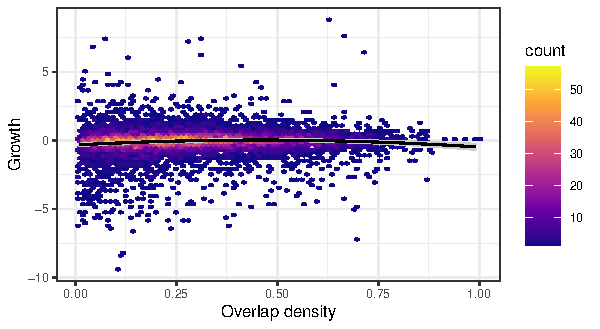
\includegraphics[width=\columnwidth]{figures/knitr-fig_densityxgrowth-1} 

\caption{A 2D histogram of subreddits with overlap density (log-transformed) on the X-axis and the change in the logarithm of the number of distinct commenting users on the Y-axis.  The black line shows the marginal effect of overlap density on growth as predicted by Model 2. The gray region shows the 95\% confidence interval of the marginal effect. \label{fig:density}}
\end{figure}

% \begin{table}
% \small
%   \centering
% <<tab.density.dependence,results='asis',echo=F,message=F>>=

% stargazer(mod.density.dependence.clusters, mod.density.avg.commensalism, mod.avg.commensalism,float=FALSE,style='apsr',keep.stat=c("n"),covariate.labels=c("Overlap density","Overlap density$^2$","Avg. subreddit mut.","Constant"),dep.var.labels=c("Growth"),dep.var.caption=NULL,no.space=TRUE,single.row=FALSE,digits=2,omit.table.layout='ld#', column.labels=c("Model 1","Model 2","Model 3"),star.cutoffs=c(0.05,0,0),notes=c("$^*$p$<0.01$"),notes.append=FALSE,add.lines=logliks)
%                                         #
% @ 
% \caption{Loglinear regression predicting subreddit growth as a function of overlap density. The model supports the prediction of density dependence theory of a $\cap$-shaped relationship between overlap density and growth. \label{tab:density}}
% \end{table}


We observe this predicted relationship between overlap density and growth. Figure \ref{fig:density} plots the marginal effects of overlap density on growth for the median subreddit laid over a scatterplot of the data.
% Table \ref{tab:density} shows regression coefficients for Models 1-3. 
%For about half of subreddits, increasing  overlap density is associated with higher growth rates.  
The point where increasing density ceases to predict increasing growth and begins to predict decreasing growth is at the 49\textsuperscript{th} percentile. 
Prototypical subreddits at this overlap density grew slightly (95\% CI:[0.001,0.06]).  Yet subreddits at the lower and upper extremes of overlap density slightly declined on average. Typical groups at the 20\textsuperscript{th} percentile of overlap density decline by 1.1 members (95\% CI:[-1.1,-1.15]) and typical groups at the 80\textsuperscript{th} percentile decline by 1.2 members (95\% CI:[-1.1,-1.28]). 

%While we find support for the classical theoretical prediction of a curvilinear, ($\cap$-shaped) relationship between overlap density and growth, this does not imply that relationships between highly overlapping communities are more competitive.  
% Instead our results below % in §\ref{sec:res.characterizing} 
% show that relationships in ecological communities of subreddits with high user overlaps are typically mutualistic. 


\subsection{Study B: Introducing Community Ecology}
\label{sec:res.characterizing}




% describe the figure and the main takeaway
% As described in §\ref{sec:characterizing.ecological.communities}, an ecological community can have positive or negative average ecological interaction §\ref{sec:mes.avg.mut} indicating if it is competitive or mutualistic and ecological interaction strength §\ref{sec:mes.abs.int}  provides a way to distinguish ecological communities with a mixture of competitive and mutualistic interactions from those where ecological interactions are weak. 

Figure \ref{fig:commense.x.abs.commense} visualizes the distribution of average ecological interaction and ecological interaction strength over the 641 ecological communities we identify.  
We observe ecological communities characterized by strong forms of both mutualism and competition, others having mixtures of the two, and some with few significant ecological interactions.  Mutualism is more common than competition, with the mean community having an average ecological interaction of 0.03 ($t=14.5$, $p<0.001$). We find that 524 clusters (81.7\%) are mutualistic. Not only are most ecological communities mutualistic, but the  ecological communities with greater mutualism have greater ecological interaction strength (Spearman's $\rho=0.58$, $p<0.001$).
% Note that due to our clustering procedure, our analysis examines ecological interactions among subreddits with relatively high degrees of user overlap.
Therefore, our community ecology analysis suggests that among groups with similar users, mutualistic ecological interactions are more common than competitive ones.

\begin{figure}

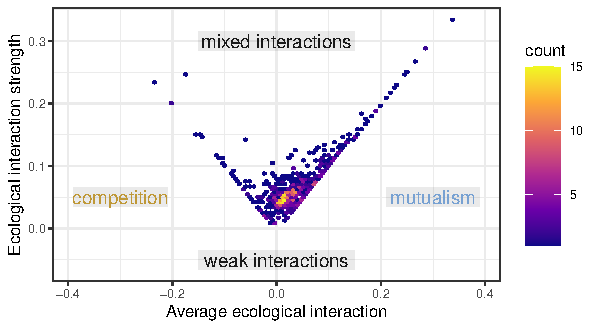
\includegraphics[width=\columnwidth]{figures/knitr-plot_commense_x_abs_commense-1} 

\caption{Two-dimensional histogram showing ecological communities on Reddit in our typology.  The X-axis shows the overall degree of mutualism or competition in clusters of subreddits with high user overlap based on the average ecological interaction.  The Y-axis shows the ecological interaction strength representing the overall magnitude of competition or mutualism.}

\label{fig:commense.x.abs.commense}
\end{figure}

\subsubsection{Example ecological communities}
\label{sec:case.studies}

We present four case studies to illustrate our typology of ecological communities of online groups.  Using our measures of average ecological interaction ($\overline{m}$) and ecological interaction strength ($\kappa$), we select cases of subreddit clusters characterized by mutualism, competition, a mixture of mutualism and competition, and few ecological relationships at all. To allow for more interesting network structures, we draw our cases from the 367 large clusters having at least five subreddits. 

\begin{figure*}
\begin{minipage}[t][][t]{1\columnwidth}
  \centering
  \hspace*{-0.1\columnwidth}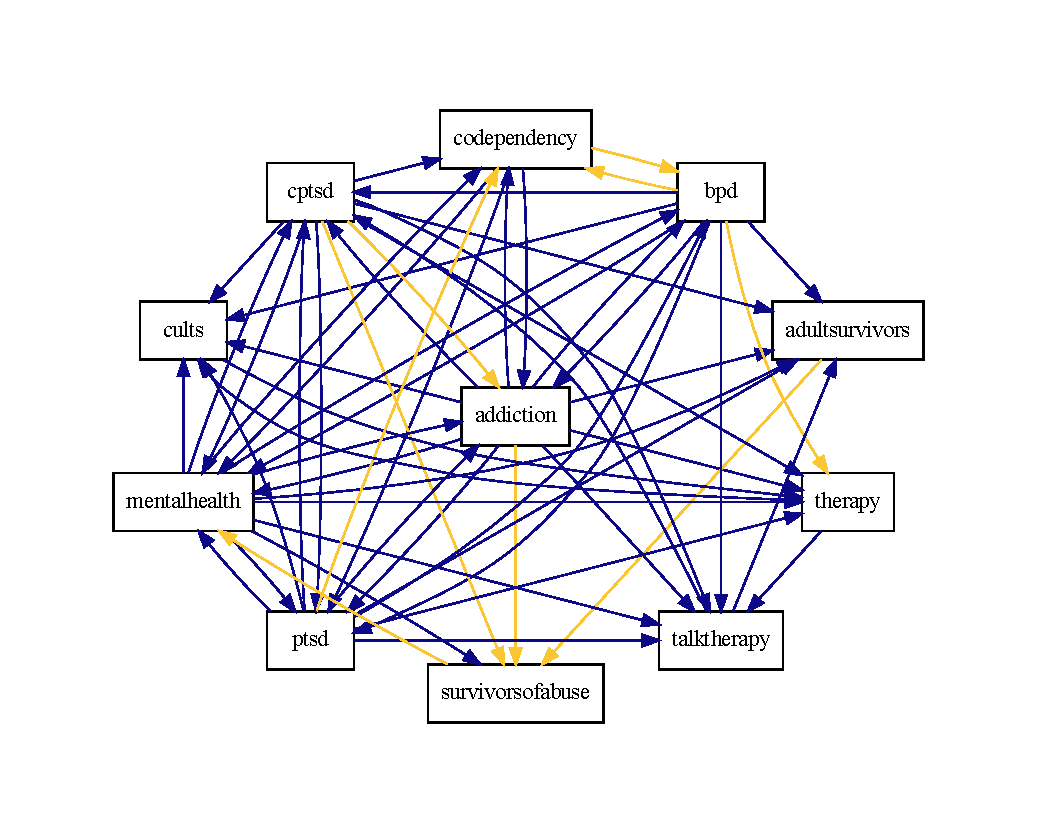
\includegraphics[width=1.2\columnwidth]{figures/mental_graphviz.pdf}
  \subcaption{The ecological community of subreddits for supporting mental health and survivors of abuse is dense with largely mutualistic interactions. 
  % Some interactions, like that between \texttt{r\Slash mentalhealth} and \texttt{r\Slash survivorsofabuse} are mutualistic in one direction but competitive in the other. 
  \label{fig:mut.network}}
\end{minipage} \hfill
\begin{minipage}[t][][t]{\columnwidth}
  \centering
  \hspace*{-0.1\columnwidth}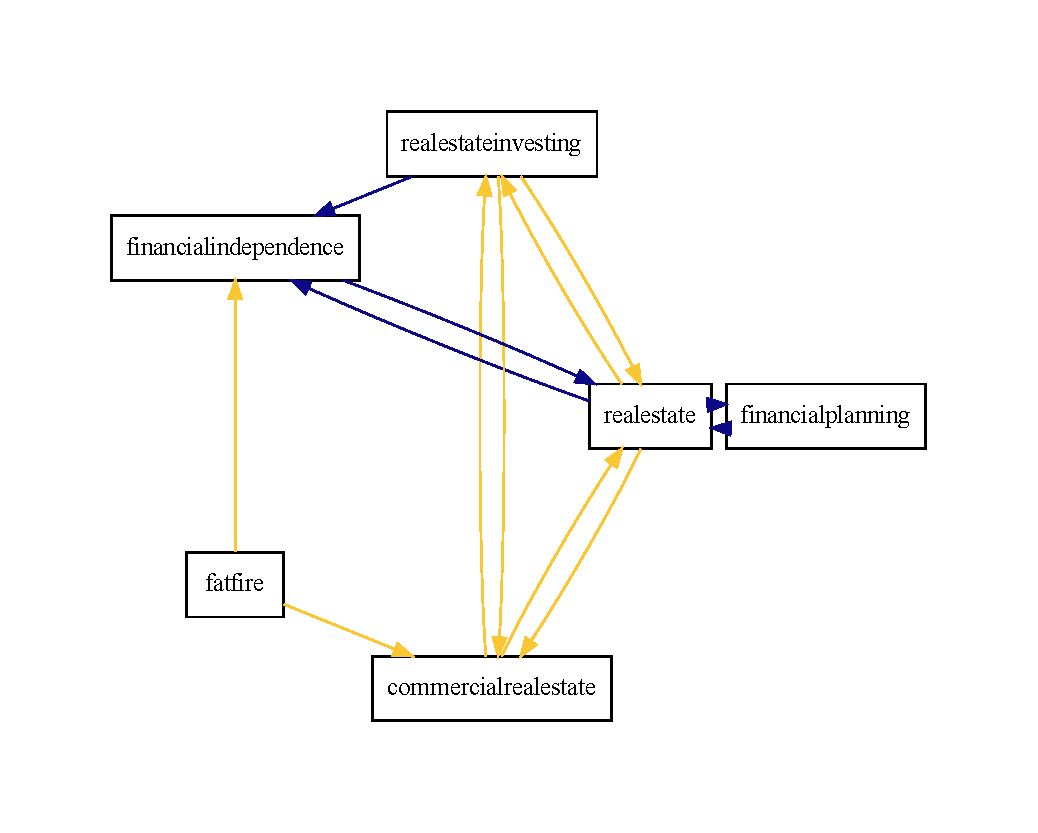
\includegraphics[width=1.2\columnwidth]{figures/realestate_graphviz.pdf}
  \subcaption{ The subreddits about real estate and finance are relatively competitive.
  % We detect reciprocal competitive relationships among the real estate subreddits in the triad including   \texttt{r\Slash realestateinvesting}, \texttt{r\Slash realestate} and \texttt{r\Slash commercialrealestate}. 
  \label{fig:comp.network}}
\end{minipage} 

\begin{minipage}[t][][t]{\columnwidth}
  \centering
  \hspace*{-0.1\columnwidth}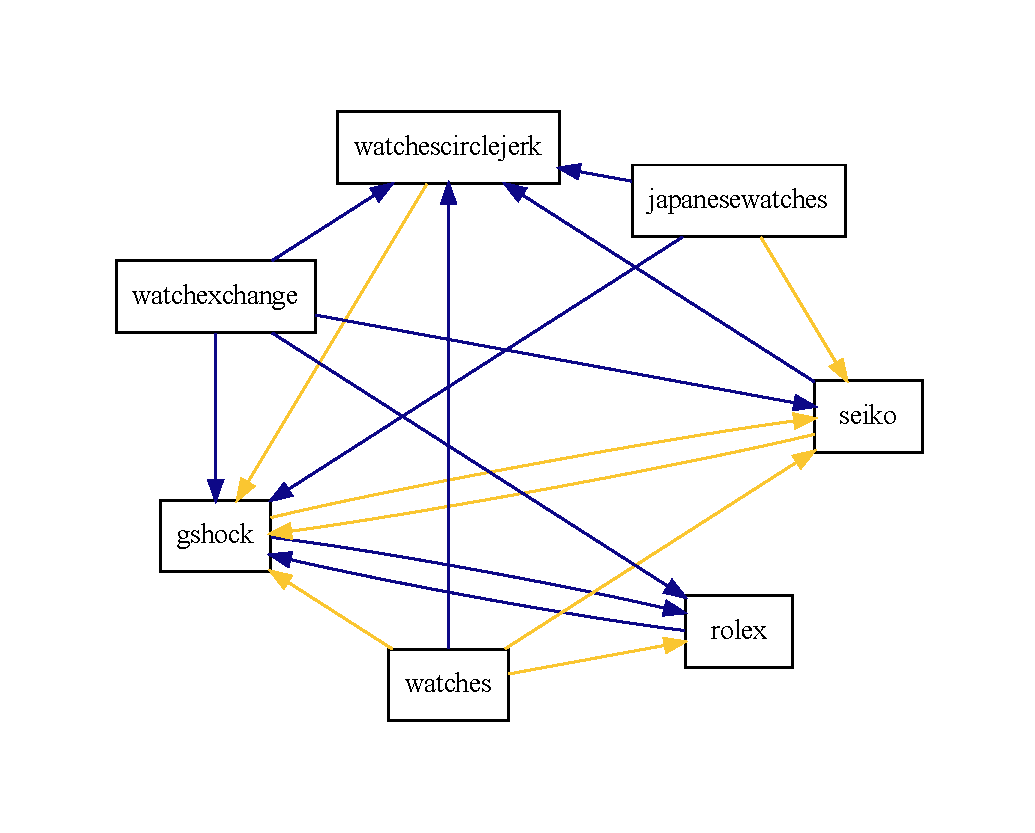
\includegraphics[width=1.2\columnwidth]{figures/watches_graphviz.pdf}
  \subcaption{Subreddits about watches are dense with both mutualistic and competitive interactions. 
  % There is a reciprocal competitive interaction between \texttt{r\Slash gshock} and \texttt{r\Slash seiko}, a reciprocal mutualistic interaction between \texttt{r\Slash gshock} and \texttt{r\Slash rolex} well as several unreciprocated mutualistic and competitive interactions.
  \label{fig:mixed.network}}
\end{minipage}
\hfill
\begin{minipage}[t][][t]{\columnwidth}
  \centering
  \hspace*{-0.1\columnwidth}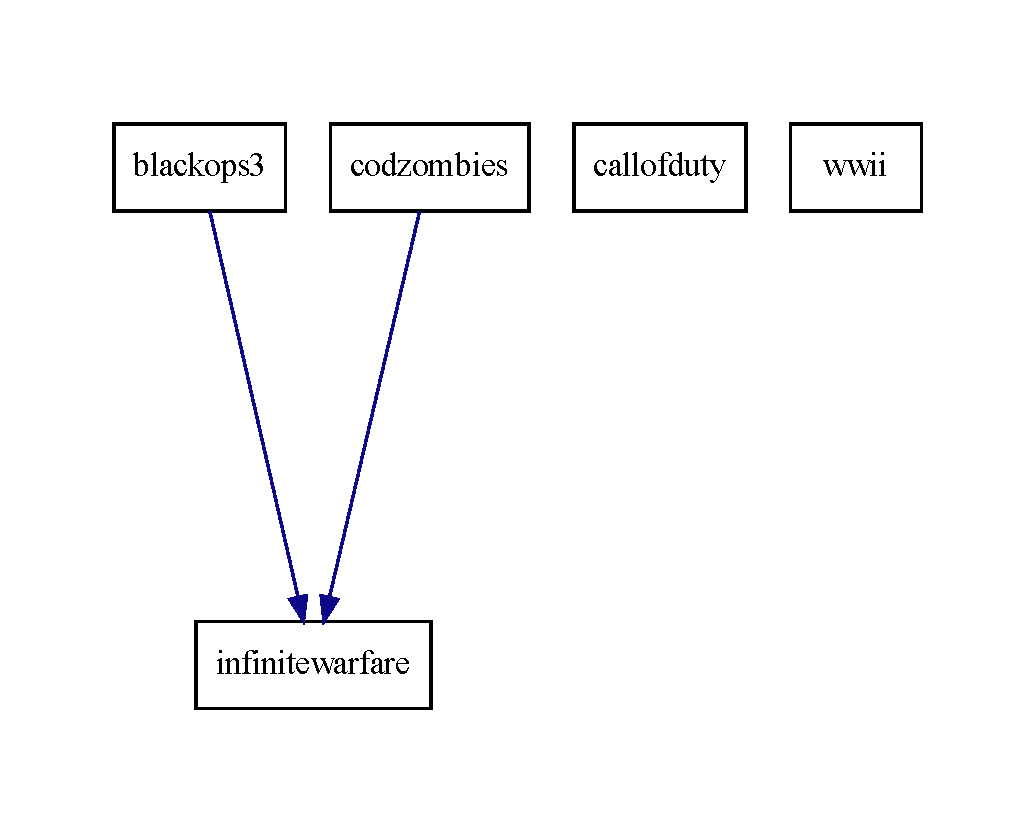
\includegraphics[width=1.2\columnwidth]{figures/cod_graphviz.pdf}
  \subcaption{The ecological community of subreddits about Call of Duty video games is characterized by relatively sparse ecological interactions.
  % We detect only two mutualistic interactions from \texttt{r\Slash blackops3} to \texttt{r\Slash infinitewarfare} from codzombies to \texttt{r\Slash infinitewarfare}. 
  \label{fig:void.network}}
\end{minipage}
\caption{Network visualizations of commensal relationships in example ecological communities of subreddits with overlapping users. Yellow indicates competition and purple indicates mutualism. \label{fig:networks}}
\end{figure*}

Figure \ref{fig:networks} presents visualizations of competition-mutualism networks that represent statistically significant impulse response functions for all relationships within our four case clusters. For each case, we examined the terms of the vector autoregression parameter $\mathbf{\Phi}$, the impulse response functions, and the model fits and forecasts, all of which are available in our online supplement.  We also visited each subreddit in the clusters and read their sidebars and top posts to support our brief qualitative descriptions.

\subsubsection{Mutualism among mental health subreddits}

% TODO, cite somebody on mental health.
To find a case characterized by mutualism, we selected the top 37 large clusters with the greatest average ecological interaction. From these, we arbitrarily chose one interesting ecological community, the \textit{mental health} cluster, which includes 11 subreddits for supporting people in struggles with mental health, addiction, and surviving abuse.  
Constitutive subreddits include those focused on specific mental health diagnoses like \texttt{r\Slash bpd} (bipolar disorder) and \texttt{r\Slash cptsd} (complex post traumatic stress disorder) while others like \texttt{r\Slash survivorsofabuse} and \texttt{r\Slash adultsurvivors}
are support groups. 

The interactions among these subreddits are dense and primarily mutualistic, as shown in Figure \ref{fig:mut.network}. There are a handful of competitive interactions like the reciprocal competition detected between \texttt{r\Slash codedependence} and \texttt{r\Slash bpd}. We also observe some interactions that are mutualistic in one direction and competitive in the other. For example, growth in \texttt{r\Slash addiction} predicts an increase in growth in \texttt{r\Slash cptsd}, even as that growth in \texttt{r\Slash cptsd} predicts a decrease in growth in \texttt{r\Slash addiction}. This suggests a pattern in which \texttt{r\Slash cptsd} siphons members from \texttt{r\Slash addiction}. That said, the density of mutualistic interactions shown in Figure \ref{fig:mut.network} suggests that different subreddits have complementary functions in this ecological community as people turn to different types of groups for help with interrelated problems.  While attempting to explain why different online groups form mutualistic or competitive interactions is left to future research, the example of mental health subreddits demonstrates how groups with related topics and overlapping participants can have mutualistic interactions.

\subsubsection{Competition among real estate and finance subreddits}

To find competitive clusters, we selected an ecological community that we label \textit{finance} from the 36 large clusters with the lowest average ecological interaction having six subreedits. Three of them: \texttt{r\Slash realestateinvesting}, \texttt{r\Slash realestate} and \texttt{r\Slash commercialrealestate}, deal with different aspects of the real estate industry, while \texttt{r\Slash financialindependence} and \texttt{r\Slash fatfire} (the acronym ``fire'' means ``financial independence/retire early'') focus on building wealth and becoming financially independent, and \texttt{r\Slash financialplanning} is a general financial advice subreddit.

Unlike the ecological community for mental health, the finance cluster has mostly competitive ties as visualized in Figure \ref{fig:comp.network}. We detect three reciprocal competitive interactions among the three subreddits that focus on real estate. The edges from \texttt{r\Slash fatfire} to \texttt{r\Slash commercialrealestate} and \texttt{r\Slash financialindependence} are also competitive.   

Although this cluster is among the most competitive in our data, it contains mutualistic ties between the general finance subreddits (\texttt{r\Slash financialplanning} and \texttt{r\Slash financialindependence}) and \texttt{r\Slash realestate}. This reflects just how prevalent mutualism is among subreddits with high degrees of user overlap. 

%  Interestingly, all interactions are mutualistic.
%Interestingly, are mutualistic.

\subsubsection{Mixed interactions among timepiece subreddits}

Next, we turn to the \textit{timepiece} ecological community of
7 subreddits about watches that has low average ecological interaction but high ecological interaction strength. 
We selected the \textit{timepiece} subreddits from the 36 %(10\%) 
large clusters with average ecological interaction closest to 0 and then from the 15 clusters with the greatest ecological interaction strength.

As shown in Figure \ref{fig:mixed.network}, the network of timepiece subreddits is dense with ecological interactions (although not as dense as the mental health subreddits). We observe both reciprocated interactions, like the mutualism between \texttt{r\Slash rolex} and \texttt{r\Slash gshock} or the competition between \texttt{r\Slash gshock} and \texttt{r\Slash seiko} and unreciprocated interactions like the mutualism between \texttt{r\Slash watchexchange} and \texttt{r\Slash watchcirclejerk}\footnote{The suffix is widely understood on Reddit to signify a jokey, meme, or satirical subreddit.}
or the competition between \texttt{r\Slash japanesewatches} and \texttt{r\Slash seiko}.
Although the average ecological interaction among these subreddits is near 0, our analysis reveals a complex ecological community with a mixture of competition and mutualism.   
 
\subsubsection{Sparse interactions among Call of Duty subreddits}

To find a case where ecological interactions are weak, we returned to the group of the 36 %(10\%) 
large clusters with average ecological interaction closest to 0 but selected from the 15 clusters within this group with the lowest ecological interaction strength. From these, we chose the \textit{Call of Duty} cluster containing five groups about the popular series of video games.

% % more quotations
The Call of Duty ecological community is sparse, having only two significant ecological interactions among its 5 member groups. This ecological community includes subreddits about different editions of the series such as \texttt{r\Slash blackops3}, \texttt{r\Slash infinitewarfar} and \texttt{r\Slash wwii} as well as one about a popular spin-off zombie game \texttt{r\Slash codzombies} and the more general \texttt{r\Slash callofduty} subreddit. We find that  growth in \texttt{r\Slash blackops3} or \texttt{r\Slash codzombies} predicts growth in \texttt{r\Slash infinitewarfare}, but no other ecological interactions. 

The timepiece and Call of Duty ecological communities illustrate how subreddits with overlapping users can have relatively strong or weak forms of ecological interdependence.  Although both clusters are characterized by high degrees of user overlap and low average ecological interaction, the timepiece cluster has a dense competition-mutualism network, while the Call of Duty network is sparse.


% \begin{wrapfigure}{l}{0.48\columnwidth}

%   \centering
%   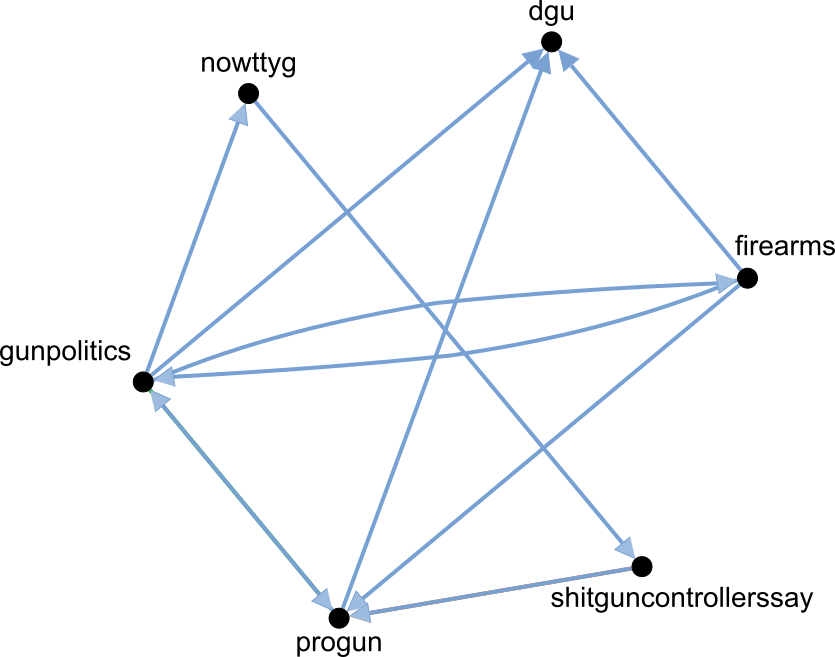
\includegraphics[width=0.48\columnwidth]{figures/gun_network.png}
%   \subcaption{An ecological community of pro-gun subreddits that is predominantly mutualistic. We detect a fully mutualistic relationship between \texttt{r\Slash firearms} and \texttt{r\Slash gunpolitics} and many partially mutualistic relationships.\label{mut.network}}
% \end{wrapfigure}

%Including VAR coefficients does not improve n.test-week forecast performance in this cluaster ($\mathrm{RMSE}_{\mathrm{base}}=round(gun.var[["ar.rmse.author_cluster_829_tf"]],2)$; $\mathrm{RMSE}_{\mathrm{var}}=round(gun.var[["var.rmse.author_cluster_829_tf"]],2)$; $\mathrm{CRPS}_{\mathrm{base}}=round(gun.var[["ar.crps.author_cluster_829_tf"]],2)$; $\mathrm{CRPS}_{\mathrm{var}}=round(gun.var[["var.crps.author_cluster_829_tf"]],2)$).  



% \begin{figure*}[t]
% \centering
% <<comp.coefs, echo=F, results='asis', fig.width=3.5, fig.height=2.5>>=
% coef <- diet.var$var.coef.author_cluster_1_tf
% ctab <- plot.coef.ols.data(coef)

% p <- dwplot(ctab)

% p <- p + scale_y_discrete(labels=parse(text=levels(ctab$term)),breaks=levels(ctab$term))
% print(p)
% @ 
% \caption{Commensal coefficients from VAR model estimated on cluster of weight-loss subreddits.}
% \end{figure*}

%Analysis of a second simulation with 15 groups and more information about our simulation studies is available in the online supplement.  

% When \citeauthor{wang_impact_2012} observes that organizations in the same population can occupy different niches, they encounter a confusion common in the application of population ecology in domains where heterogeneity between organizations is salient: \emph{what is a niche} anyway?  

% In translating ecological concepts from biology to organizations many organizational ecologists came to see organizations as individuals belonging to populations.  This was a fruitful choice for looking at relatively homogeneous industries such as newspapers  
    
% it's very important that individual communities are seen as different.


% 1 longish paragraphs ~ 200 words summarizing empirical findings of interdependence between online communities

% Approaches to interdependence between online communities
    
% Population vs Community Ecology
    
% Inference of ecological relationships


% containing \emph{overlap density} terms alone may not explain much variance in subreddit growth among the nrow(df) subreddits that were assigned to clusters (R$^2$ = signif(summary(mod.density.dependence)[["r.squared"]],1)).  Neither does \emph{average subreddit commensalism} (R$^2$ = signif(summary(mod.avg.commensalism)[["r.squared"]],1)).
  
    
% \subsection{Study C: Predicting Growth}
% \label{sec:res.studyC}

% We now compare the environmental approach of population ecology with the relational approach of community ecology.
% In Study B, we presented examples of diverse ecological communities among subreddits with overlapping members.  However, the presence of this diversity this does not mean that ecological interactions are related to the growth of online groups, the key outcome of previous ecological studies.  We therefore hypothesized that ecological interactions will improve the predictive performance of a density dependence model in H2.

% \subsubsection{Ecological interactions do not improve growth prediction}
% \label{sec:res.likelihood.ratio.test}

% To test H2, we compare Model 1, our density dependence model having first- and second-order terms for overlap density, with Model 2, which also includes average subreddit mutualism (§\ref{sec:mes.sub.mut}) as a predictor.  We also examine Model 3, in which the only predictor is average subreddit mutualism. Table \ref{tab:density} shows regression coefficients for our models. 

% We do not observe a statistically significant association between average subreddit mutualism and growth ($B_3=round(coef(mod.density.avg.commensalism)[['avg.subreddit.commensalism']],2), SE=round(coef(summary(mod.density.avg.commensalism))[,'Std. Error'][["avg.subreddit.commensalism"]],2)$).  
% % We observe that average subreddit mutualism is positively associated with growth , which makes sense as subreddits with greater average subreddit mutualism benefit more from mutualism or are hurt less from competition.
% Moreover, a likelihood ratio test comparing Model 1 and Model 2 does not support H2 as Model 2 does not predict subreddit growth better than Model 1 ($\chi^2 = signif(test.1[["Chisq"]][2],2)$, $p>0.05$). 
% % Therefore, average subreddit mutualism does not help predict growth compared to the density dependence model alone. 
% Comparing Model 2 to Model 3 shows that overlap density explains variation that average subreddit mutualism does not ($\chi^2 = signif(test.2[["Chisq"]][2],2)$, $p<0.001$). 
% %This suggests that the density of a subreddit's niche helps explain subreddit growth in important ways not captured by ecological interactions.  
% Overlap density helps explain a group's future growth, but the overall degree of mutualism or competition a group faces in its ecological community does not. 
% % In §\ref{sec:discussion}, we discuss how overlap density may only capture the hospitality of a group's environment and may be independent of mutualism and competition within its ecological community.
 
\subsubsection{Forecasting accuracy}
\label{sec:res.forecasting}

% The likelihood ratio tests in §\ref{sec:res.likelihood.ratio.test} are limited because improvements in predictive performance (or lack thereof) may be due to unobserved factors predictive of growth that are correlated with average subreddit mutualism. 
 
% We hypothesized in H2 that the intergroup dependencies in our VAR models can better forecast the size of subreddits compared to baseline time series models that do not account for ecological interactions.  

We test H2 using two metrics of whether we have improved the 24-week forecast performance for all  subreddits which were assigned to clusters: root-mean-square-error (RMSE) and continuous ranked probability score (CRPS).
We find that VAR models including ecological interactions have better forecasting performance than the baseline model in terms of both. The RMSE under the baseline model (0.84) is greater than the RMSE of the VAR models (0.75) and the CRPS of the baseline model (72,853) is   greater than the CRPS of the VAR models (72,669).
% This reflects a substantive improvement in forecast accuracy robust to the choice of the forecasting metric.  

% Our baseline model contains a constant term and a trend term for each group and therefore accounts for all time-invariant within-group variation.  Because overlap density is a subreddit-level variable that does not vary over time,
% we know that the improvement in forecasting performance comes from modeling ecological interactions in ways not captured by overlap density.

\section{Threats to Validity}
\label{sec:limitations}
Our work is subject to several important threats to validity. First, we study only one platform hosting online groups, and our results may not generalize to other platforms or time periods.
The method we propose for identifying ecological interactions between online groups has limitations common to all time series analysis of observational data. 
While our community ecology approach assumes that ecological interactions drive dynamics in the size of groups over time and cause groups to grow or decline, drawing causal conclusions using our method would depend on several untestable assumptions. For example, groups we do not consider---including groups on other platforms---could affect ecological communities in ways unaccounted for in our models.  Potential omitted variables may also include additional time lags of group size.  We chose to use VAR(1) models with a single time lag for simplicity, but we hope future work will model more complex dynamics with additional lags.

Our vector autoregression models assume that the error terms are trend stationary. This is a common assumption in time series analysis and is difficult to evaluate empirically  \cite{ives_estimating_2003}. 
Future work might relax these assumptions using sophisticated models or additional contextual knowledge of ecological communities of interest. 
Such models may also be useful in future work investigating how ecological interactions change over time.

Additional threats to validity stem from our use of algorithmic clustering to identify ecological communities.
While we choose clusters based on high degrees of user overlap and validate our clustering, we might have obtained different results if we had clustered in a different way. Additionally, our efforts to obtain clusters with a high silhouette coefficient led us to remove subreddits from our analysis. Thus, our results are not representative of Reddit in general, but only of those subreddits that were included in our analysis.
Furthermore, clustering algorithms may not have unique solutions, and different initial conditions can lead to different results. 

% Clustering enabled us to perform a broad analysis, but future work should conduct narrow analysis of important ecological communities defined using principled definitions and qualitative contextual knowledge.

Organizational ecologists have rarely attempted to estimate the full community matrix for an entire population containing a large number of groups because of data and statistical limitations \cite[e.g.][]{ruef_emergence_2000, sorensen_recruitment-based_2004}. For instance, there are nearly 100 million possible ecological interactions among 10,000 communities.  Attempting to infer all of them raises considerable computational and statistical challenges.
This makes it necessary to narrow the scope to the ecological communities of interest in ways appropriate to the research question.
We clustered communities according to user overlap in order to explore typical ecological communities on a platform, but future investigations should consider other quantitative or qualitative approaches to constructing ecological communities.

% Yet, a 
 % Finally, our three cases studies are limited in that they can offer only a proof-of-concept analysis and an enticing hint at more comprehensive future analyses with more rigorously defined populations of online groups.
% Although we found varying results in the three ecological communities we selected, these case studies can provide little explanation for when one should expect to find different forms of commensalism in online groups. Our hope is that these initial results can point in new directions for research. 
% % We looked at three different sets of related online groups and found three qualitatively different ecological communities.  
% As is true in all case study research, there is little reason to expect findings from any one of our case studies to generalize to any specific other set of contexts.

\section{Discussion}
\label{sec:discussion}
In the final chapter of their book on \textit{Building Successful Online Communities}, \citet{kraut_building_2012} advise managers of online groups to select an effective niche and beware of competition. However, these recommendations are based on little direct evidence from studies of online groups and offer almost no concrete steps that a designer or group should take based on either piece of advice. Although further research into ecological interactions is needed to derive design principles, we provide a novel framework for online group managers to think about ecological constraints on group size. 
Intuition suggests that online group managers might seek mutualistic relationships and avoid competitive ones, but it is not clear whether another group is a competitor or mutualist. Our method provides a way for group managers to know. 

We presented two studies with the purpose of introducing our community ecology framework and comparing it with previous work using population ecology.
In Study A, we found support for H1 by showing---as predicted by density dependence theory---that overlap density has an $\cap$-shaped association with subreddit growth.
Subreddits with moderate overlap density in our data declined less than subreddits with either very low or very high overlap density. According to population ecology theory, this suggests that high-density environments are competitive and less conducive to growth than medium-density environments.

%prevalence of mutualism among highly overlapping subreddits contrast with our results for
Surprisingly, this seems to contrast with our results in Study B. When we studied ecological communities using vector autoregression models of group size over time to infer networks of ecological interactions, 
we found that ecological communities of subreddits are typically mutualistic and that these mutualistic interactions are stronger on average than competitive ones.
These findings corroborate recent qualitative studies arguing that multiple online communities about the same topic exist because they provide different and complementary benefits \cite{teblunthuis_no_2022}, such as those provided by combinations of small and large subreddits \cite{hwang_why_2021}.
Moreover, we found support for H2 by showing that the ecological interactions in these models are useful for forecasting group size. This validates our inferences of ecological interactions and provides compelling evidence that ecological interactions are an important factor affecting the development of online communities. 


We also found a diversity of ecological dynamics among clusters of subreddits with high degrees of user overlap. We found ecological communities that are mutualistic, competitive, that mix the two or that have few significant ecological interactions at all. 
This explains the puzzling set of empirical results from previous work on the relationship between overlap density and outcomes like growth, decline and survival  \cite{wang_impact_2012, zhu_impact_2014, zhu_selecting_2014}.
These studies have measured the density of an online group's niche in terms of its overlap in participants or topics. 
Although we find support for the relationship between density and growth predicted by density dependence theory, our analysis of ecological communities suggests that degrees of overlap may have little to do with whether two groups are mutualists or competitors. 

By correlating an online communities' aggregated resource overlaps to their growth or survival, tests of density dependence theory obscure complex networks of ecological relationships.
As a result, interpreting these correlations as evidence that pairs of groups with the greatest resource overlaps are most likely to compete commits an ecological fallacy \citep{piantadosi_ecological_1988, robinson_ecological_1950}.  
Our method provides a path for future work to understand the relationship between resource overlaps and ecological interactions by directly inferring when groups are competitors or mutualists instead of relying on aggregations. 

That said, we believe that density dependence models can usefully reflect environmental conditions.  Density is associated with growth when a platform provides a hospitable environment to build online communities that share certain topics or membership bases. 
Yet, when conditions change and these topics lose popularity or membership bases migrate off a platform \cite{fiesler_moving_2020}, density can become associated with decline. 
For example, the differing environmental conditions of Wikia wikis and Usenet groups might explain why user overlap was associated with the survival of wikis \cite{zhu_impact_2014} but with the decline of Usenet groups \cite{wang_impact_2012}. Wikia was a young and growing platform during \citepos{zhu_impact_2014} data collection period when the growth of groups may have been limited by knowledge of how organize and build a wiki; perhaps this knowledge was provided by overlapping experienced members. 
Usenet was in decline during \citepos{wang_impact_2012} study period and this may have created competition over increasingly scarce members. 

Future work should seek to explain when two online groups will be mutualists or competitors. 
Long-held understandings of ecological interactions in evolutionary theory suggest that, as we find, mutualism will be more common than competition \cite{kropotkin_mutual_2012}. 
Competition is unlikely to persist because it decreases survival; but mutualistic relationships are likely to endure because they increase it.
In this line of theory, groups might avoid competition by adopting specialized functions in their ecological communities, a dynamic known as resource partitioning  \cite{carroll_concentration_1985}. For example, the competition among the real estate subreddits observed in Figure \ref{fig:comp.network} may occur due to insufficient specialization.  
% If specialization does not emerge over time, groups of competing subreddits may have decreased survival. 
By contrast, mental health support groups such as those observed in Figure \ref{fig:comp.network} appear to have specialized purposes or functions. 

%Future work should test such mechanisms may explain when competition and mutualism will manifest within ecological communities in online platforms. 

Online groups may use multiple platforms with distinctive affordances for different purposes \cite{kiene_technological_2019}. 
Since our VAR method relies only on time series data to infer ecological interactions, it can be applied to study ecological communities spanning social media platforms. 
% Community ecology can thus provide a bridge between quantitative studies of participation in online groups and theories of interconnected information ecologies \cite{nardi_information_1999}. 
While we focus on relationships between groups sharing a platform, one can apply our concepts and methods to understand how higher levels of social organization emerge from interdependent systems of technologies and users on social media platforms. 
% Finally, future work should conduct studies of important cases of ecological communities engaged in peer production, political mobilization, misinformation, or mental health support. 

\section{Conclusion}

% Rewrite conclusion
An ecological explanation for the success of online groups looks beyond internal mechanisms to understand how different groups influence each other's growth or decline.
Prior research has investigated competition and mutualism among online groups with overlapping users and topics using the population ecology framework \cite{wang_impact_2012, zhu_impact_2014, zhu_selecting_2014}, yet has not provided a way to infer competitive or mutualistic interactions among related groups.
We introduce the community ecology framework as a complementary perspective to population ecology. 
% The two ecologies both seek to explain why online groups grow or survive, but they focus on different levels of analysis \cite{astley_two_1985}.  
By inferring competition-mutualism networks directly from time series data, our community ecology approach helps resolve the empirical tensions raised by prior work and reveals that most interactions within clusters of highly overlapping subreddits are mutualistic. 
Our methods provide a foundation for future work investigating related online groups.  

\section*{Ethics Statement}

The intended broader impact of this work is to improve the design and management of online communities by advancing scientific understanding of overlapping communities.  It is conceivable that this work could contribute to potential harms, such as if it is used to organize socially harmful online communities.  We hope and believe that any negative consequences of this work will be outweighed by positive and productive ones. We are sensitive to the ethical concerns about large-scale analysis of publicly available social media communication and behavior, such as ours, in that the individuals whose traces we analyze are unlikely to anticipate their data will be used in such a way. That said, because our analysis aggregates these activities to such a degree that no individual is exposed to scrutiny, we believe that the resulting harms are minimal. We have no competing financial interests in this work.

\section*{Code and Data Availability}

Supplementary material, as well as the code and data to replicate this analysis, is available via the Harvard Dataverse at \url{https://doi.org/10.7910/DVN/KLGHKY}.

\section*{Acknowledgments}
Text from a draft of this article was included as part of the first authors PhD dissertation and he thanks his committee---Professors Kirsten Foot, Aaron Shaw, David McDonald and Emma Spiro,  for their generous support, wise advice and insightful comments. 
Versions of this paper received very helpful feedback at the  International Communication Association's 2021 annual meeting. We are thankful to the Community Data Science Collective for additional feedback and Sohyeon Hwang, Jeremy Foote,  Carl Colglazier, and Kaylea Champion in particular.

We owe special gratitude to Daryn McElroy for her work to externally validate our clusters.
Thank you to Jason Baumgartner and pushshift.io for the Reddit data archive.
Also, we thank to the peer reviewers whose insightful comments improved the quality of this article. Any remaining errors and imperfections are ours.  
This work was supported by NSF grants IIS-1908850 and IIS-1910202 and GRFP \#2016220885 and was facilitated through the use of the advanced computational infrastructure provided by the Hyak supercomputer system at the University of Washington.

%Resource overlaps seem to reflect competitive forces in some circumstances but mutualistic ones in others. 
%surveyed clusters of highly overlapping groups on Reddit to.
%As discussed more below, our results are due to the fact that support for H1 does not necessarily mean that most relationships between subreddits with the greatest degrees of user overlap are competitive.
% We demonstrate that the size of the other members of  ecological community improves time series forecasts of participation in online groups. 
% However, average subreddit mutualism did not help predict growth. This suggests that population ecology and community ecology offer complementary environmental and relational perspectives.   
% Population ecology's focus on environmental factors such as niche and overlap density is useful for predicting growth, but does not provide a way to study networks of mutualism and competition.
% Community ecology unpacks density and provides insights about the specific relationships between groups.  


% While modeling these interactions helps forecast participation levels in groups, the existence of these interactions may be independent of future growth. 
% For example, if mutualistic relationships are common in declining ecological communities, that would explain our result for H2.

%  these interactions helps time series forecasting, but whether the interactions 

% While we advance community ecology as an alternative framework to population ecology, our results show that population ecology and community ecology are complementary perspectives. 
% We tested H2 to find out whether including subreddit average mutualism improves the ability of a density dependence model to predict the size of a subreddit n.test weeks in the future and found that it did not. Therefore,

% Yet in support of H3, including ecological interactions in the vector autoregression (VAR) models substantially improves their forecasting performance. 
 

% Our  findings in Study A and Study B may appear contradictory, their coincidence in our data points to ways in which population ecology and community ecology conceive of different kinds of ecological dynamics. 
%Users of groups with high overlap density may have greater commitment to the platform than to any particular group and competition over such users may become fierce when a platform goes into decline. 

% as users with comm

% because 

% and \citeauthor{tan_all_2015} \cite{tan_all_2015} observe that accounts posting in fewer different groups are more likely to leave a platform.  
% As \citeauthor{kraut_building_2012} \cite{kraut_building_2012} argue, commitment to subgroups can enhance commitment to a broader group.  This suggests that On the other hand, members of a group with high overlap density may have little commitment to it in particular.  

% This suggests that commitment to a 

% We suggest that when commitment to the platform declines this may amplify competition as 
% may present environmental conditions for strong competition over those members  
% This suggests that 
% Such groups may face greater challenges in sustaining participation when the platform goes into decline. 

%Our results demonstrate population ecology's approach to competition and mutualism in a test of density dependence theory and provide an evaluation of community ecology's ability to predict subreddit growth.


%Future work should directly test this hypothesis about the relationships between platform-based and subgroup-based commitment.

% In general, competition over overlapping resources will have no effect on group growth if something besides the overlapping resource limits growth \cite{verhoef_community_2010}. For example, two wikis might share a large number of contributors (have high user overlap), but their growth might be limited by a lack of core contributors who perform important administrative tasks like policy making and software administration \cite{zhu_impact_2014}.   Community ecology relaxes the assumption that competition and mutualism are caused by user overlap density and instead seeks to infer them from data.
% To illustrate our approach, we presented 4 example ecological communities found on Reddit §\ref{sec:case.studies}.

% Methods from network science might be used to construct and test  theories about the roles of different types of resources, design features of platforms, and governance institutions in these ecological interactions. 


% Within large platforms for online groups, the great number of ecological communities that can be studied should make it possible for future work to apply 


% \subsection{Implications for Design}
    
% While Resnick et al.~\citep{resnick_starting_2012} 

% Competitors have a negative impact on growth, but ecological theory suggests that specialization is an adaptive strategy in response to competition \cite{carroll_concentration_1985}. 
% %For example, the growth of Wikipedia caused other online encyclopedia projects to shift their focus \cite{hill_almost_2013}. 
% Using our method, group managers might identify competitors limiting the growth of their groups. With the knowledge of this analysis in hand, they might be able to escape a competitive dynamic by specializing. 
% While competitive relationships are defined by how they decrease the size of groups, competition can also be important to the health of the broader ecological community. Exit to an alternative group can be an avenue for political change in response to grievances and poor governance \cite{hirschman_exit_1970, frey_emergence_2019}. The threat of competition with other groups may make expressions of voice more persuasive to moderators or platforms \cite{hirschman_exit_1970}. 
% Groups looking to increase activity should desire to seek out mutualistic relationships, and we believe that designers of online platforms can help them do so. Features such as meta-groups, group search, recommendation engines, and practices like linking related groups may lower barriers between groups and support mutualism. However, it is not obvious to what extent particular features will support competition, mutualism, or both.  Using our method, managers and designers can test features intended to support mutualism.




% \bibliographystyle{ACM-Reference-Format}
\bibliography{ecological_models}



\end{document}
\endinput
%% LOCALWORDS autoregression
%% End of file `sample-authordraft.tex'.
%People regularly participate in multiple online communities \cite{fara}. While online communities often have well-defined topical boundaries, these boundaries can overlap and shift \cite{butler_cross-purposes_2011}. 
    
\subsection{Sketching a chart of the ecological frontier}
    
Community ecology of offline organizations emphasizes how the evolution of ties in a network shapes the development of industries \cite[e.g.][]{dimaggio_social_2001, monge_evolutionary_2011, monge_communication_2008}.  
    
Organizational scholars 
    

Active cooperation by communities may be an important form of mutualism that can be cultivated through new designs. While the commensal relationships we study may arise from patterns in how individuals choose to participate in communities, they may also form intentionally as two communities intentionally collaborate or when a new community forms in order to compete with an old one.  


\subsection{Inferring the community matrix for social computing systems} 


Most VAR models in macroeconomics and biological ecology are fit using ordinary least squares, an approach which relies on assumptions that will be difficult to sustain in the online group settings of our interest. The number of parameters in the model increases quadratically with the number of variables in the system which can lead to over-fitting, estimation difficulties, and false discoveries arising from the testing of a large number of hypotheses. 

%For models fit using OLS, non-normal errors can lead to bias. A Bayesian vector autoregression approach can overcome such limitations and allows the use of hierarchical priors that pull estimates towards 0 and thereby correct for multiple hypothesis tests  \cite{canova_bayesian_2007, banbura_large_2010, gelman_why_2012}.  

%We extend Equation \ref{eq:var1} to include a Poisson link function and a hierarchical Bayesian prior structure. We use a Poisson link function in order to model count data for groups with smaller numbers of participants.  In our model, $Y_t$ is a count of participants distributed according to Poisson parameter $\lambda_t$ which has a multivariate normal distribution evolving over time according to a VAR process. The parameter $\Phi$ corresponds to the community matrix as described in \textsection \ref{sec:var}. We use $X_{t}$ to account for seasonality as described in our case studies.  

We use impulse response functions to quantify how much a group's size will change in response to a sudden increase in the size of another group represented by $\Theta_0$, which is an identity matrix so our impulses represent a log-unit increase of 1. Our models have a latent VAR process which we transform into a count variable through a Poisson link.  To interpret IRFs in terms of the number of members of a group, we transform them using a baseline of the median number of participants in a group over the study period, ($\widetilde{Y}_i$) and exponentiating to obtain $\Theta_i^*$ as shown in Equation \ref{eq:irf}. 

\begin{align}
    \Theta_i &= \Theta_{i-1}\mathbf{\Phi}, i = 1,2,... \label{eq:irf} \\
    \Theta_i^* &= e^{\Theta_i + \mathrm{log}(\widetilde{Y}_i)} \nonumber
\end{align}

Stationarity is a common assumption in time series analysis \cite{ives_estimating_2003}. For a VAR(1) model, stationarity means assuming that the eigenvalues of $\mathbf{\Phi}$ are all less than 1. Practically speaking, this assumes that groups will not grow infinitely nor that the probabilities of activity in them will go to zero. In developing our model, we found that enforcing stationarity through the Heaps prior improved forecast accuracy and helped us fit larger VAR models including more online groups \cite{heaps_enforcing_2020}.  More information on our models, including our prior specifications is available in Appendix \ref{ap:model}.
We developed our model using the Stan probabilistic programming language building off of code published by \citet{heaps_enforcing_2020} to add support for intercept terms, account for seasonality, and count data \cite{carpenter_stan:_2016}. In our simulation and in all our empirical case studies we report results from Stan models fit using 4 chains that pass Stan's diagnostic checks.  We have released all code and data necessary to reproduce these analysis in the Harvard Dataverse.


%Our intervention is to directly infer ecological relationships in networks of related communities through the framework of community ecology. In doing so, we make both theoretical and methodological contributions to social computing scholarship. 

%analyzes \emph{ecological communities} comprised of heterogeneous and interdependent groups \citep{astley_two_1985}. 

% In biology, this might be different populations of organisms inhabiting a lake or valley. In organization science, this might be the network of technology developers, manufacturers, and suppliers in the semiconductor industry \cite{powell_network_2005, verhoef_community_2010}. Community ecology is also of considerable influence in organization science \citep[e.g.][]{astley_two_1985, margolin_normative_2012, ruef_emergence_2000, powell_network_2005, monge_evolution_2008, barnett_competition_1987}, but to our knowledge, community ecology has never been applied in social computing research.


%on how environmental factors shape the dynamics within a population such as a biological species.
% (e.g., bats of species \emph{Myotis lucifugus} in biology) 
% (e.g. newspapers in organizational ecology).
%The earliest and most influential works of ecology as applied to human organizations used the population ecology approach to answer questions such as those about how organizational forms become established or decline \cite{aldrich_organizations_2006}. This approach requires treating a population as consisting of entities with similar resource needs while ignoring the distinct roles that individual groups play.
%Population ecology has framed every ecological analysis of online groups published in social computing venues that we are aware of. 

% Thinking about backing off somewhat from "mired in confusion"

% Thinking about removing "ecological fallacy" in par below
% \citeauthor{zhu_selecting_2014} \cite{zhu_selecting_2014}  finds support of this theoretical prediction. However, studies in other settings find weak or theoretically inconsistent relationships \cite{tan_tracing_2018, teblunthuis_population_2020}. By focusing on resources overlaps like topical similarity and shared participants,  \citet{wang_impact_2012}, \citet{zhu_selecting_2014}, and \citet{zhu_impact_2014} all study the role of dyadic relationships between online groups in their growth or decline. 

%In order to advance project of advancing community ecology in social computing we compare and contrast it with the population ecology approach. In §\ref{sec:density} we report an original population ecology analysis on our dataset from Reddit. 

% At this point we have built up the intuition of DDT, but now we will sow doubt in it and build up the intuition of the alternative community ecology.



% The inconsistent findings in the population ecology of online groups might be explained if user overlaps suggest that groups interact but have little to do with whether they are mutualists or competitors. For instance, perhaps most ecological interactions among overlapping Wikis were mutualistic in \citepos{zhu_impact_2014} context but were competitive in \citepos{wang_impact_2012} owing to differences in the resources needs of Wikis and Usenet groups. Wikia was a growing platform during \citepos{zhu_impact_2014} data collection period. Perhaps they found increased survival among new communities with overlapping members from established groups because the growth of groups was limited by knowledge of how to build a wiki and this knowledge was provided by more experienced users. Usenet was in decline during \citepos{wang_impact_2012} study period and it may not have been limited in this way.


% Paragraph explaining why we find so much mutualism in terms of resource partitioning theory and specialization.

% Paragraph suggesting future work explore apply methods of network analysis to these inferred networks to understand the roles that different communities play in their ecosystems1. 



    

%n an ecological community focused on Seattle, we find a great number of mutualistic relationships. Among groups for sharing wallpaper images, we found almost no commensal relationships.  In design and craft humor subreddits we find many mutualistic ties, but also predation, and no commensal ties between those groups where visibly posted norms clearly distinguished between content xappropriate for sharing in each group. 

%While our case studies reveal variation in networks of commensal relationships between related groups, case studies alone cannot resolve the puzzle of why resource overlaps appear related to competition in some circumstances \cite{teblunthuis_population_2020,wang_impact_2012} but in others appear related to mutualism \cite{zhu_impact_2014,zhu_selecting_2014}. However our results provide strong support for the claim that relationships between similar communities might be competitive or mutualistic depending on factors other than content or topical overlaps.

% Future studies should investigate such aspects of the dynamics between  governance and commensalism.

% Finally, we propose that future work investigates higher-level properties of ecological communities.  The motivation for community ecology is not only to better describe commensal relationships between online groups, but also to better understand how groups shape one another as well as higher order social structures like social media platforms and technological cultures.  

%we can also conceive of studies of relationships between different populations of groups such as populations defined by groups located on different social media platforms. 

%Studying relationships between populations raises challenges of measurement and data collection not faced by studies of groups within the same platform
%  collective decision making to shift topic, policies, or governance practices. 

%One direction toward such ends is to analyze stability dynamics of VAR models to investigate conditions giving rise to relatively stable or unstable ecological communities in social computing systems \cite{ives_estimating_2003}.

%Approaching interdependence between online groups from a community ecology perspective means recognizing relationships between groups and the networks formed from these relationships in ecological communities as an object of study in their own right. 

%We observe a fully mutualistic relationship between the two subreddits that share a general scope of ``gun politics:'' \texttt{r\Slash progun} and \texttt{r\Slash gunpolitics}. This means that an increase in the size of \texttt{r\Slash progun} predicts a subsequent increase in the size of \texttt{r\Slash gunpolitics} and that growth in \texttt{r\Slash gunpolitics} predicts growth in \texttt{r\Slash progun}. There is a second fully mutualistic relationship between \texttt{r\Slash gunpolitics} and \texttt{r\Slash firearms}, another generalist subreddit that contains political content.

% All of the remaining subreddits have specialized focuses related to pro-gun information. We observe many partially mutualistic relationships among them. \texttt{r/nowttyg} is an acronym for ``no one wants to take your guns'' and exists to detail ``evidence contradicting the gun control movements claim that they merely seek moderate'' proposals that don't involve the seizure of existing firearms.  It has a partially mutualistic relationships with \texttt{r/shitguncontrollerssay}, such that growth in \texttt{r/nowtyg} predicts growth in \texttt{\Slash r\Slash shit\-gun\-con\-trol\-lers\-say}.  \texttt{r/firearms}, \texttt{r/progun}, and \texttt{r/gunpolitics} all have partially mutualistic relationships benefiting \texttt{r/dgu}, which stands for ``defensive gun use'' and which is ``dedicated to cataloging incidents in the United States where legally owned or legally possessed guns are used by civilians to deter or stop crime.''  

%  \texttt{r/b} is specifically for ``improvised armed vehicles'' which are defined as ``are makeshift/homemade vehicles that have been modified with weapons and armour,'' while \texttt{r/tanks} and \texttt{r/tankporn} have photography of more conventional modern and historical military vehicles. The other two subreddits in the group are about video games with realistic gameplay emphasizing military vehicles.


% While growth far from the only criteria of success for an online group, much social computing research follows RDT by seeking to support groups' growth and survival through the attraction or retention of members \cite{koh_encouraging_2007, kraut_role_2014, cunha_are_2019}. 

% For example, explanations of Wikipedia's transition from growth to decline  structures for quality assurance in a growing project that constituted barriers to newcomer participation \cite{halfaker_rise_2013, teblunthuis_revisiting_2018} spawned significant interest in designs for increasing newcomer retention that have met with limited success \citep[e.g.][]{halfaker_snuggle:_2014, morgan_tea_2013, narayan_wikipedia_2017}. Social structures like leadership, organizational practices, network structure, and design decisions can lower costs and increase benefits of participation \cite{butler_membership_2001, kraut_role_2014, tsugawa_impact_2019}. 


%TODO: incorporate the below citations to "demonstrate that this is of importance to the social computing audience""  Also cite Charlie's paper about cross-platform interdependence

%We review this foundational work in §\ref{sec:resource_dep} and then narrow our focus to prior ecological studies and other empirical work about interdependence between online groups in §\ref{sec:ecology_background}. Then, in §\ref{sec:community_ecology} we review sociological research developing community ecology theory and apply it to online groups.  
  
% It also builds closely on two bodies of ecological theory: first, explanations from population ecology that describe entities as sharing resources in environments and second, explanations from community ecology that theorize networks of specific community relationships.
% In our background we introduce the first two bodies of related work in sections \ref{sec:resource_dep} and \ref{sec:ecology_background}.
    
    % Frame around the dependent variable: 
    
    % Explaining participation is important because 
    % 1. It's a longstanding concern of the field
    % 2. Online Groups are important to society  
    % models 
    % ranging from entertainment, information exchange, social interaction, to the collaborative production of knowledge and organization of collective action


% This positive feedback between the value of prior contributions and the motivation for future contributions drives community growth.  
% Think about the implications of our findings for the rival vs nonrival resources that could be in play.

% Maybe try to deepen the discussion of resource competition, or maybe its better to avoid getting dragged into this.



% Online participation in general has opportunity costs and may compete with alternatives like sleep, entertainment, or work \cite{becker_theory_1965, butler_attraction-selection-attrition_2014}.
% So online groups that provide similar benefits may be the most likely competitors because once someone has obtained satisfying benefits from one group they may go offline or switch to another activity instead of seeking similar benefits from competitor groups.\footnote{Economists refer to these as ``substitutes.' }

% providing the same benefits at lesser costs might be a compelling alternative.
% If different online groups can substitute for participation in one another and participation is rival this will lead to competition between the communities and decrease participation in both.
% Public goods are nonrival because their usefulness is not diminished when others use them.

